
%% bare_conf.tex
%% V1.4b
%% 2015/08/26
%% by Michael Shell
%% See:
%% http://www.michaelshell.org/
%% for current contact information.
%%
%% This is a skeleton file demonstrating the use of IEEEtran.cls
%% (requires IEEEtran.cls version 1.8b or later) with an IEEE
%% conference paper.
%%
%% Support sites:
%% http://www.michaelshell.org/tex/ieeetran/
%% http://www.ctan.org/pkg/ieeetran
%% and
%% http://www.ieee.org/

%%*************************************************************************
%% Legal Notice:
%% This code is offered as-is without any warranty either expressed or
%% implied; without even the implied warranty of MERCHANTABILITY or
%% FITNESS FOR A PARTICULAR PURPOSE! 
%% User assumes all risk.
%% In no event shall the IEEE or any contributor to this code be liable for
%% any damages or losses, including, but not limited to, incidental,
%% consequential, or any other damages, resulting from the use or misuse
%% of any information contained here.
%%
%% All comments are the opinions of their respective authors and are not
%% necessarily endorsed by the IEEE.
%%
%% This work is distributed under the LaTeX Project Public License (LPPL)
%% ( http://www.latex-project.org/ ) version 1.3, and may be freely used,
%% distributed and modified. A copy of the LPPL, version 1.3, is included
%% in the base LaTeX documentation of all distributions of LaTeX released
%% 2003/12/01 or later.
%% Retain all contribution notices and credits.
%% ** Modified files should be clearly indicated as such, including  **
%% ** renaming them and changing author support contact information. **
%%*************************************************************************


% *** Authors should verify (and, if needed, correct) their LaTeX system  ***
% *** with the testflow diagnostic prior to trusting their LaTeX platform ***
% *** with production work. The IEEE's font choices and paper sizes can   ***
% *** trigger bugs that do not appear when using other class files.       ***                          ***
% The testflow support page is at:
% http://www.michaelshell.org/tex/testflow/



\documentclass[conference]{IEEEtran}
% Some Computer Society conferences also require the compsoc mode option,
% but others use the standard conference format.
%
% If IEEEtran.cls has not been installed into the LaTeX system files,
% manually specify the path to it like:
% \documentclass[conference]{../sty/IEEEtran}



\usepackage{algorithm}
\usepackage{algorithmic}
\usepackage{graphicx}
\usepackage{amsmath}
\usepackage{multirow}
% Some very useful LaTeX packages include:
% (uncomment the ones you want to load)


% *** MISC UTILITY PACKAGES ***
%
%\usepackage{ifpdf}
% Heiko Oberdiek's ifpdf.sty is very useful if you need conditional
% compilation based on whether the output is pdf or dvi.
% usage:
% \ifpdf
%   % pdf code
% \else
%   % dvi code
% \fi
% The latest version of ifpdf.sty can be obtained from:
% http://www.ctan.org/pkg/ifpdf
% Also, note that IEEEtran.cls V1.7 and later provides a builtin
% \ifCLASSINFOpdf conditional that works the same way.
% When switching from latex to pdflatex and vice-versa, the compiler may
% have to be run twice to clear warning/error messages.



% *** CITATION PACKAGES ***
%
%\usepackage{cite}
% cite.sty was written by Donald Arseneau
% V1.6 and later of IEEEtran pre-defines the format of the cite.sty package
% \cite{} output to follow that of the IEEE. Loading the cite package will
% result in citation numbers being automatically sorted and properly
% "compressed/ranged". e.g., [1], [9], [2], [7], [5], [6] without using
% cite.sty will become [1], [2], [5]--[7], [9] using cite.sty. cite.sty's
% \cite will automatically add leading space, if needed. Use cite.sty's
% noadjust option (cite.sty V3.8 and later) if you want to turn this off
% such as if a citation ever needs to be enclosed in parenthesis.
% cite.sty is already installed on most LaTeX systems. Be sure and use
% version 5.0 (2009-03-20) and later if using hyperref.sty.
% The latest version can be obtained at:
% http://www.ctan.org/pkg/cite
% The documentation is contained in the cite.sty file itself.






% *** GRAPHICS RELATED PACKAGES ***
%
\ifCLASSINFOpdf
  % \usepackage[pdftex]{graphicx}
  % declare the path(s) where your graphic files are
  % \graphicspath{{../pdf/}{../jpeg/}}
  % and their extensions so you won't have to specify these with
  % every instance of \includegraphics
  % \DeclareGraphicsExtensions{.pdf,.jpeg,.png}
\else
  % or other class option (dvipsone, dvipdf, if not using dvips). graphicx
  % will default to the driver specified in the system graphics.cfg if no
  % driver is specified.
  % \usepackage[dvips]{graphicx}
  % declare the path(s) where your graphic files are
  % \graphicspath{{../eps/}}
  % and their extensions so you won't have to specify these with
  % every instance of \includegraphics
  % \DeclareGraphicsExtensions{.eps}
\fi
% graphicx was written by David Carlisle and Sebastian Rahtz. It is
% required if you want graphics, photos, etc. graphicx.sty is already
% installed on most LaTeX systems. The latest version and documentation
% can be obtained at: 
% http://www.ctan.org/pkg/graphicx
% Another good source of documentation is "Using Imported Graphics in
% LaTeX2e" by Keith Reckdahl which can be found at:
% http://www.ctan.org/pkg/epslatex
%
% latex, and pdflatex in dvi mode, support graphics in encapsulated
% postscript (.eps) format. pdflatex in pdf mode supports graphics
% in .pdf, .jpeg, .png and .mps (metapost) formats. Users should ensure
% that all non-photo figures use a vector format (.eps, .pdf, .mps) and
% not a bitmapped formats (.jpeg, .png). The IEEE frowns on bitmapped formats
% which can result in "jaggedy"/blurry rendering of lines and letters as
% well as large increases in file sizes.
%
% You can find documentation about the pdfTeX application at:
% http://www.tug.org/applications/pdftex





% *** MATH PACKAGES ***
%
%\usepackage{amsmath}
% A popular package from the American Mathematical Society that provides
% many useful and powerful commands for dealing with mathematics.
%
% Note that the amsmath package sets \interdisplaylinepenalty to 10000
% thus preventing page breaks from occurring within multiline equations. Use:
%\interdisplaylinepenalty=2500
% after loading amsmath to restore such page breaks as IEEEtran.cls normally
% does. amsmath.sty is already installed on most LaTeX systems. The latest
% version and documentation can be obtained at:
% http://www.ctan.org/pkg/amsmath





% *** SPECIALIZED LIST PACKAGES ***
%
% \usepackage{algorithmic}
% algorithmic.sty was written by Peter Williams and Rogerio Brito.
% This package provides an algorithmic environment fo describing algorithms.
% You can use the algorithmic environment in-text or within a figure
% environment to provide for a floating algorithm. Do NOT use the algorithm
% floating environment provided by algorithm.sty (by the same authors) or
% algorithm2e.sty (by Christophe Fiorio) as the IEEE does not use dedicated
% algorithm float types and packages that provide these will not provide
% correct IEEE style captions. The latest version and documentation of
% algorithmic.sty can be obtained at:
% http://www.ctan.org/pkg/algorithms
% Also of interest may be the (relatively newer and more customizable)
% algorithmicx.sty package by Szasz Janos:
% http://www.ctan.org/pkg/algorithmicx




% *** ALIGNMENT PACKAGES ***
%
%\usepackage{array}
% Frank Mittelbach's and David Carlisle's array.sty patches and improves
% the standard LaTeX2e array and tabular environments to provide better
% appearance and additional user controls. As the default LaTeX2e table
% generation code is lacking to the point of almost being broken with
% respect to the quality of the end results, all users are strongly
% advised to use an enhanced (at the very least that provided by array.sty)
% set of table tools. array.sty is already installed on most systems. The
% latest version and documentation can be obtained at:
% http://www.ctan.org/pkg/array


% IEEEtran contains the IEEEeqnarray family of commands that can be used to
% generate multiline equations as well as matrices, tables, etc., of high
% quality.

% *** SUBFIGURE PACKAGES ***
%\ifCLASSOPTIONcompsoc
%  \usepackage[caption=false,font=normalsize,labelfont=sf,textfont=sf]{subfig}
%\else
%  \usepackage[caption=false,font=footnotesize]{subfig}
%\fi
% subfig.sty, written by Steven Douglas Cochran, is the modern replacement
% for subfigure.sty, the latter of which is no longer maintained and is
% incompatible with some LaTeX packages including fixltx2e. However,
% subfig.sty requires and automatically loads Axel Sommerfeldt's caption.sty
% which will override IEEEtran.cls' handling of captions and this will result
% in non-IEEE style figure/table captions. To prevent this problem, be sure
% and invoke subfig.sty's "caption=false" package option (available since
% subfig.sty version 1.3, 2005/06/28) as this is will preserve IEEEtran.cls
% handling of captions.
% Note that the Computer Society format requires a larger sans serif font
% than the serif footnote size font used in traditional IEEE formatting
% and thus the need to invoke different subfig.sty package options depending
% on whether compsoc mode has been enabled.
%
% The latest version and documentation of subfig.sty can be obtained at:
% http://www.ctan.org/pkg/subfig




% *** FLOAT PACKAGES ***
%
%\usepackage{fixltx2e}
% fixltx2e, the successor to the earlier fix2col.sty, was written by
% Frank Mittelbach and David Carlisle. This package corrects a few problems
% in the LaTeX2e kernel, the most notable of which is that in current
% LaTeX2e releases, the ordering of single and double column floats is not
% guaranteed to be preserved. Thus, an unpatched LaTeX2e can allow a
% single column figure to be placed prior to an earlier double column
% figure.
% Be aware that LaTeX2e kernels dated 2015 and later have fixltx2e.sty's
% corrections already built into the system in which case a warning will
% be issued if an attempt is made to load fixltx2e.sty as it is no longer
% needed.
% The latest version and documentation can be found at:
% http://www.ctan.org/pkg/fixltx2e


%\usepackage{stfloats}
% stfloats.sty was written by Sigitas Tolusis. This package gives LaTeX2e
% the ability to do double column floats at the bottom of the page as well
% as the top. (e.g., "\begin{figure*}[!b]" is not normally possible in
% LaTeX2e). It also provides a command:
%\fnbelowfloat
% to enable the placement of footnotes below bottom floats (the standard
% LaTeX2e kernel puts them above bottom floats). This is an invasive package
% which rewrites many portions of the LaTeX2e float routines. It may not work
% with other packages that modify the LaTeX2e float routines. The latest
% version and documentation can be obtained at:
% http://www.ctan.org/pkg/stfloats
% Do not use the stfloats baselinefloat ability as the IEEE does not allow
% \baselineskip to stretch. Authors submitting work to the IEEE should note
% that the IEEE rarely uses double column equations and that authors should try
% to avoid such use. Do not be tempted to use the cuted.sty or midfloat.sty
% packages (also by Sigitas Tolusis) as the IEEE does not format its papers in
% such ways.
% Do not attempt to use stfloats with fixltx2e as they are incompatible.
% Instead, use Morten Hogholm'a dblfloatfix which combines the features
% of both fixltx2e and stfloats:
%
% \usepackage{dblfloatfix}
% The latest version can be found at:
% http://www.ctan.org/pkg/dblfloatfix




% *** PDF, URL AND HYPERLINK PACKAGES ***
%
%\usepackage{url}
% url.sty was written by Donald Arseneau. It provides better support for
% handling and breaking URLs. url.sty is already installed on most LaTeX
% systems. The latest version and documentation can be obtained at:
% http://www.ctan.org/pkg/url
% Basically, \url{my_url_here}.




% *** Do not adjust lengths that control margins, column widths, etc. ***
% *** Do not use packages that alter fonts (such as pslatex).         ***
% There should be no need to do such things with IEEEtran.cls V1.6 and later.
% (Unless specifically asked to do so by the journal or conference you plan
% to submit to, of course. )


% correct bad hyphenation here
\hyphenation{op-tical net-works semi-conduc-tor}


\begin{document}
%
% paper title
% Titles are generally capitalized except for words such as a, an, and, as,
% at, but, by, for, in, nor, of, on, or, the, to and up, which are usually
% not capitalized unless they are the first or last word of the title.
% Linebreaks \\ can be used within to get better formatting as desired.
% Do not put math or special symbols in the title.
\title{Static Scheduling of a Time-Triggered Network-On-Chip based on Memetic Algorithm}


% author names and affiliations
% use a multiple column layout for up to three different
% affiliations
\author{
	\IEEEauthorblockN{Heyuan Shi}
	\IEEEauthorblockA{School of Software\\
	Tsinghua University\\
	Beijing, China\\
	Email: hey.shi@foxmail.com}
}

% conference papers do not typically use \thanks and this command
% is locked out in conference mode. If really needed, such as for
% the acknowledgment of grants, issue a \IEEEoverridecommandlockouts
% after \documentclass

% for over three affiliations, or if they all won't fit within the width
% of the page, use this alternative format:
% 
%\author{\IEEEauthorblockN{Michael Shell\IEEEauthorrefmark{1},
%Homer Simpson\IEEEauthorrefmark{2},
%James Kirk\IEEEauthorrefmark{3}, 
%Montgomery Scott\IEEEauthorrefmark{3} and
%Eldon Tyrell\IEEEauthorrefmark{4}}
%\IEEEauthorblockA{\IEEEauthorrefmark{1}School of Electrical and Computer Engineering\\
%Georgia Institute of Technology,
%Atlanta, Georgia 30332--0250\\ Email: see http://www.michaelshell.org/contact.html}
%\IEEEauthorblockA{\IEEEauthorrefmark{2}Twentieth Century Fox, Springfield, USA\\
%Email: homer@thesimpsons.com}
%\IEEEauthorblockA{\IEEEauthorrefmark{3}Starfleet Academy, San Francisco, California 96678-2391\\
%Telephone: (800) 555--1212, Fax: (888) 555--1212}
%\IEEEauthorblockA{\IEEEauthorrefmark{4}Tyrell Inc., 123 Replicant Street, Los Angeles, California 90210--4321}}




% use for special paper notices
%\IEEEspecialpapernotice{(Invited Paper)}




% make the title area
\maketitle

% As a general rule, do not put math, special symbols or citations
% in the abstract
\begin{abstract}
Time-Triggered Network-on-Chip (TTNoC) is one of the practical applications of real-time systems, focused on the reliable and safety-critical communication, for modern multiprocessor system. The TTNoC allows designer to achieve communication with more nodes and messages, but the scheduling of each message is a challenging problem because designer must consider both path contention and the temporal constrains. We introduce a genetic algorithm, and then integrate local search into the genetic algorithm, so called memetic algorithm, with stochastic ranking strategy to solve this problem. The experimental results show that the better performance of our memetic algorithm in compare with genetic algorithm.
\end{abstract}
% no keywords

% For peer review papers, you can put extra information on the cover
% page as needed:
% \ifCLASSOPTIONpeerreview
% \begin{center} \bfseries EDICS Category: 3-BBND \end{center}
% \fi
%
% For peerreview papers, this IEEEtran command inserts a page break and
% creates the second title. It will be ignored for other modes.
\IEEEpeerreviewmaketitle



\section{INTRODUCTION}
Many safety-critical real-time embedded systems desire the predictable communication latency. The temporal constrains of system must be guaranteed \cite{DBLP:conf/date/HuangBRBK12}. Time-Triggered system is one of the real-time architectures which isolate the inherent fault and meet the temporal predictability of communication. Therefore, Time-Triggered Network-on-Chip (TTNoC) is efficient and ideal for safety-related embedded systems because it satisfies the strict timing and dependability requirements~\cite{DBLP:journals/afp/Noce16}.

At present, time-triggered communication comes in various fields. e.g. SAFEbus deployed in the avionic industry [], TTP and FlexRay adopted in automotive  [] and TTEthernet in the domain of railway industry []. In particular, many time-triggered Networks-on-Chip architectures have been proposed (e.g., GENESYS MPSoC, Aethereal \cite{DBLP:conf/dac/2010}).

A traditional time-triggered architecture is bus-based system where all messages are scheduled in time slots and for every time slot, there is only one message which can be transmitted. To design such systems, the designer pays attention to the time domain to guarantee that all messages are non-overlapping in time domain. Each message owns its unique offset time point. In this case, a feasible schedule is an order for messages such that no two messages can be sent at the same time. 

The Time-Triggered Network-on-Chip has been proposed because the current bus-based time triggered systems cannot meet the requirements of development of Multiprocessor System-on-Chip (MPSoC) []. While NoCs provide more link resources to forward messages, it is more complex to synthesize a feasible scheduling for TTNoC since the conflict-free paths through the network-on-a-chip must be considered. The TTNoC allows several message to be transmitted at the same time slot, if their routing paths are non-overlapping. It entails messages share the time slot on the TTNoC. In this case, the designer must consider the feasible scheduling of messages in both time-domain and space-domain. In other words, any two messages cannot occupy the same network link at the identical time point. If messages coexist in time slot, the forwarding path of these messages should be conflict-free. If messages are using identical link to be forwarded, the existence time of these messages cannot be overlapped.

\begin{figure}[!t]
	\centering
	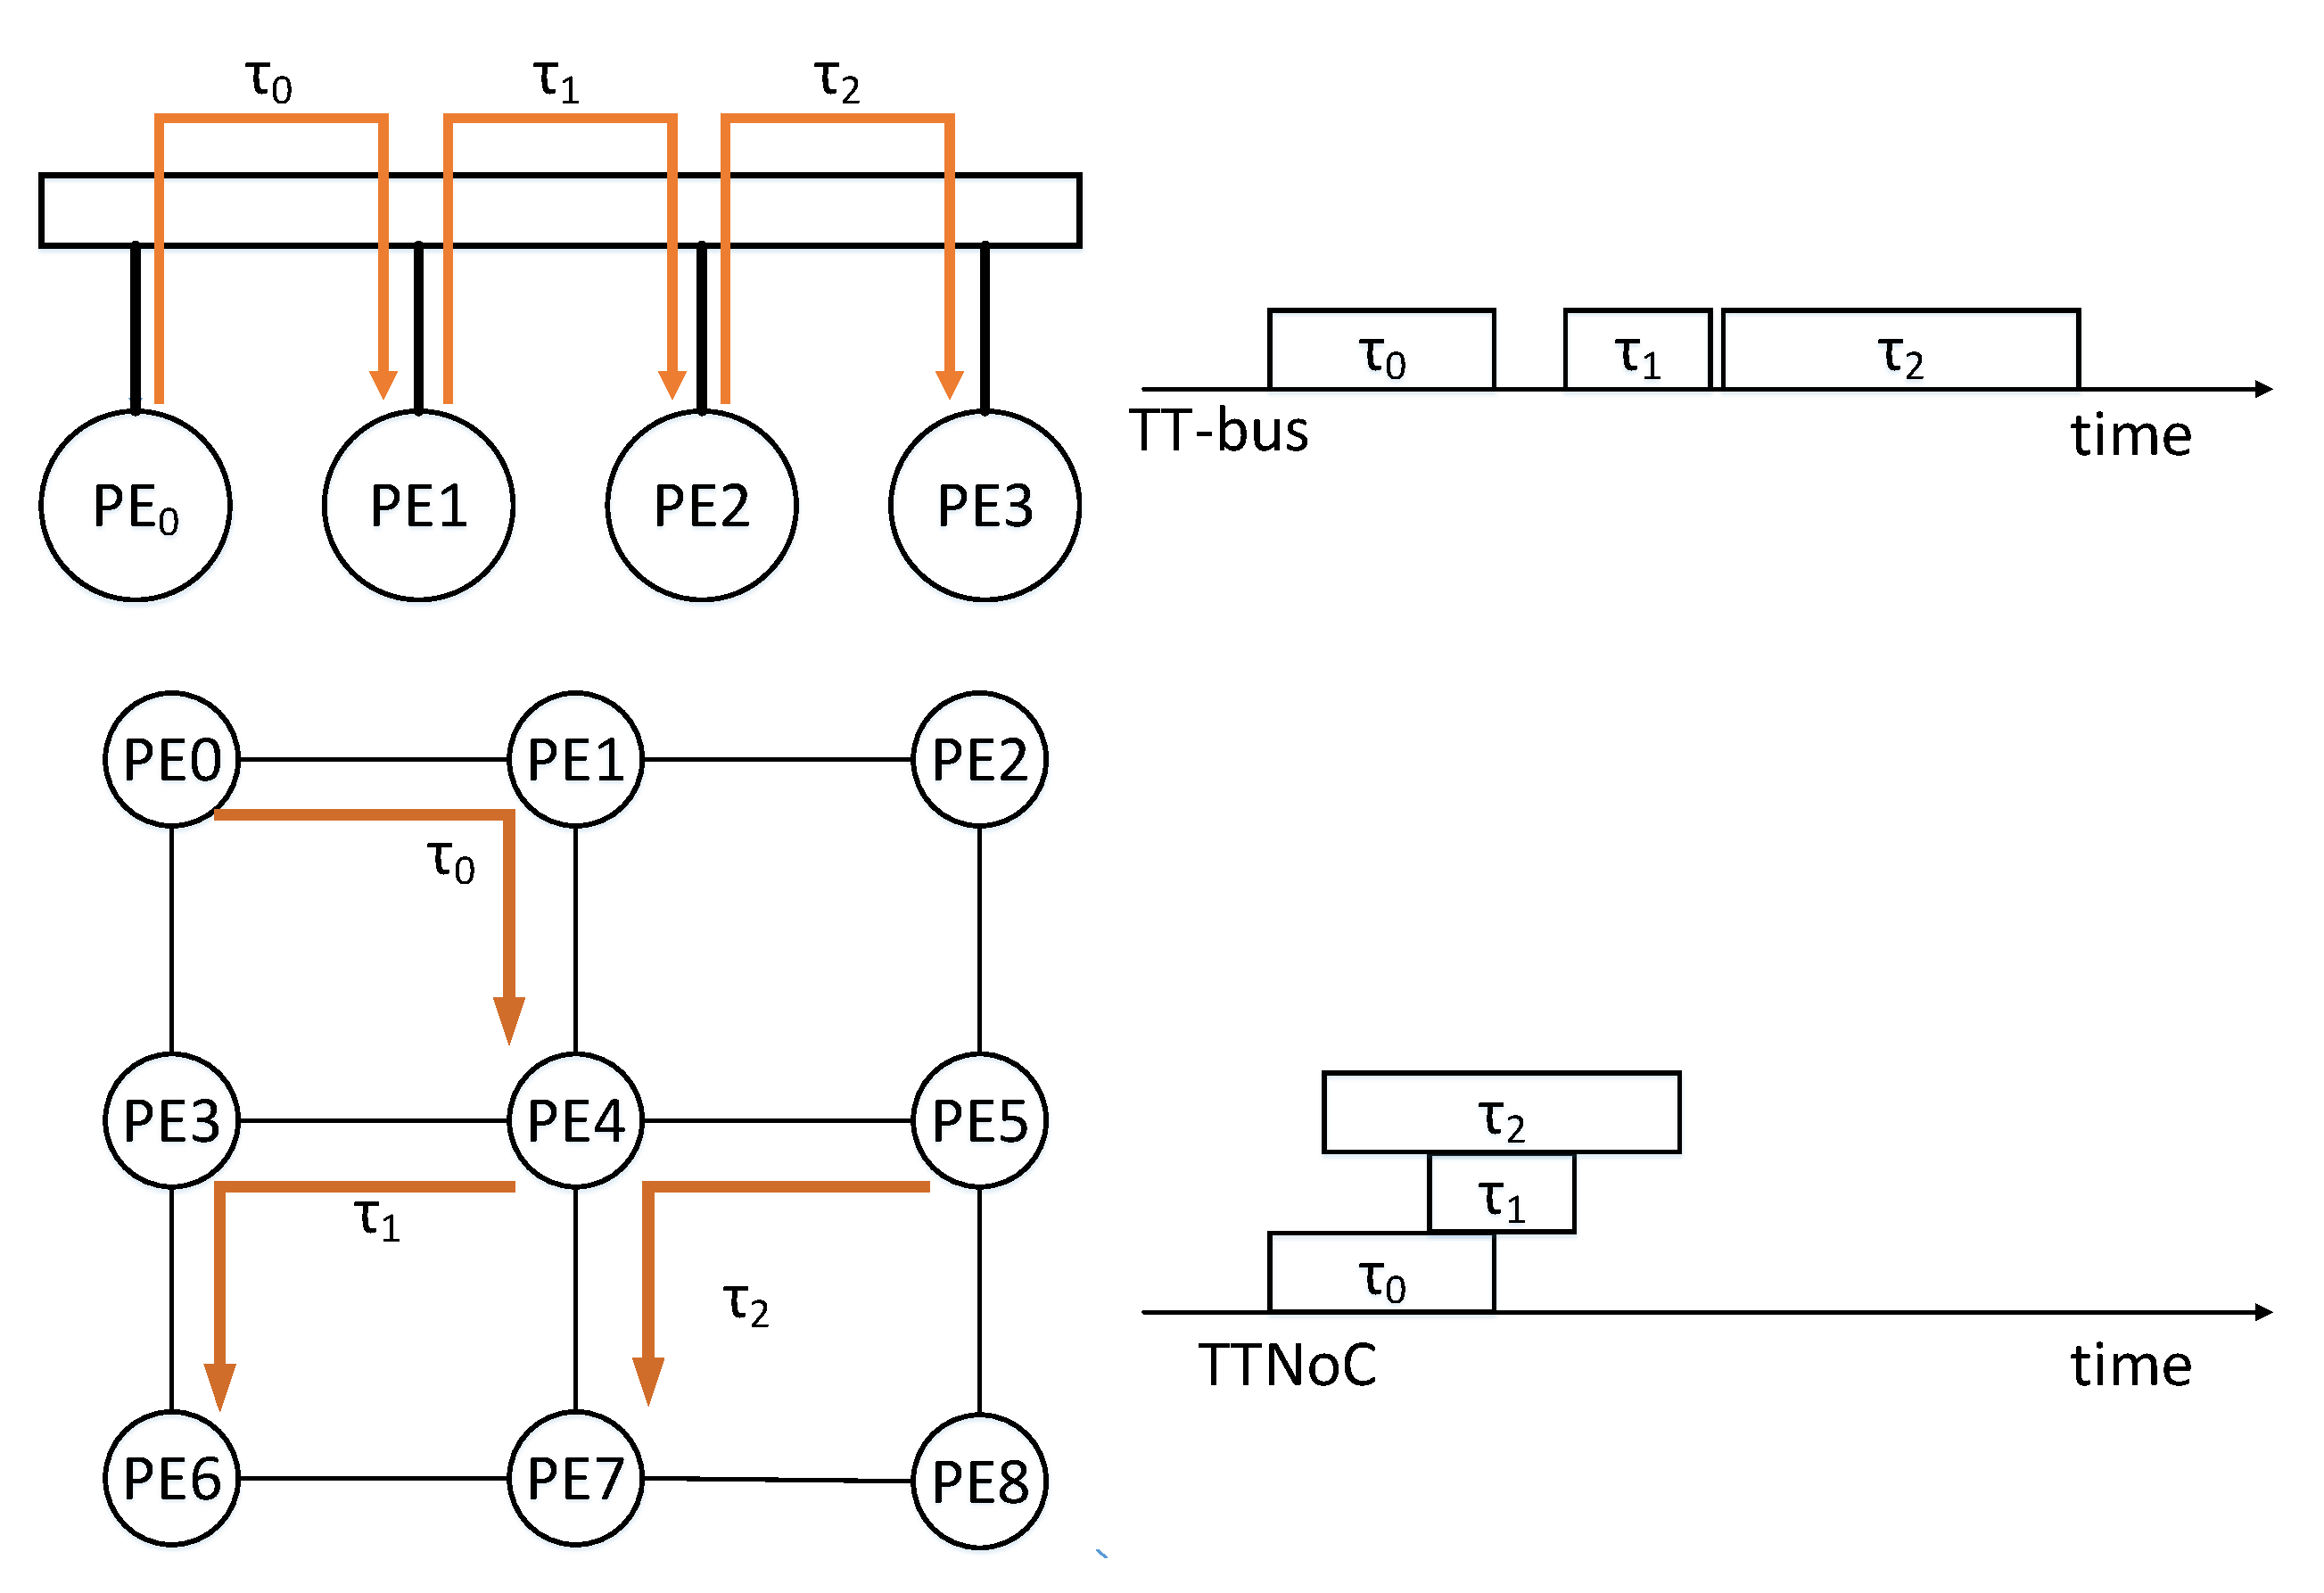
\includegraphics[width=2.5in]{picture/difference.pdf}
	\caption{Difference between bus- and network-based time-triggered architecture}
	\label{f:arch}
\end{figure}

Time-Triggered system resolves contention on the network and avoids dynamic arbitration of intercommunicate resources distribution by the synchronizing time of communication entities and static schedule upon the global synchronized time []. With the control of a global time imposed by the system, the local time of every node on the chip is synchronized to each other. The offset time point of each message (the injection of each messages), from any nodes on the network, is defined by a static schedule table, and the switches on the network also transmit the messages in terms of the schedule table. Therefore, all the messages are received, transmitted or sent at a deterministic time point with the correctness and predictability of real-time communication. However, synthesizing such an off-line schedule table is rather complicated which is viewed as a bin-packing problem, known as NP-complete [].

This paper presents a static scheduling approach to solve the TTNoC scheduling problem by the Memetic Algorithm. Memetic Algorithm is widely used as a synergy of evolutionary or any population-based approach with separate individual learning or local improvement procedures for problem search. 

The rest of this paper is organized as follows. We first review the related work in the TTNoC scheduling Section II. The problem definition and the constrains about the problem (Section III). Then the memetic algorithm with stochastic ranking has been proposed to find the feasible solution (Section IV). Finally, the memetic algorithm was implemented to compare with other SMT-based static scheduling approaches, and the related discussion was also included (Section V).

% An example of a floating figure using the graphicx package.
% Note that \label must occur AFTER (or within) \caption.
% For figures, \caption should occur after the \includegraphics.
% Note that IEEEtran v1.7 and later has special internal code that
% is designed to preserve the operation of \label within \caption
% even when the captionsoff option is in effect. However, because
% of issues like this, it may be the safest practice to put all your
% \label just after \caption rather than within \caption{}.
%
% Reminder: the "draftcls" or "draftclsnofoot", not "draft", class
% option should be used if it is desired that the figures are to be
% displayed while in draft mode.
%
%\begin{figure}[!t]
%\centering
%\includegraphics[width=2.5in]{myfigure}
% where an .eps filename suffix will be assumed under latex, 
% and a .pdf suffix will be assumed for pdflatex; or what has been declared
% via \DeclareGraphicsExtensions.
%\caption{Simulation results for the network.}
%\label{fig_sim}
%\end{figure}

% Note that the IEEE typically puts floats only at the top, even when this
% results in a large percentage of a column being occupied by floats.


% An example of a double column floating figure using two subfigures.
% (The subfig.sty package must be loaded for this to work.)
% The subfigure \label commands are set within each subfloat command,
% and the \label for the overall figure must come after \caption.
% \hfil is used as a separator to get equal spacing.
% Watch out that the combined width of all the subfigures on a 
% line do not exceed the text width or a line break will occur.
%
%\begin{figure*}[!t]
%\centering
%\subfloat[Case I]{\includegraphics[width=2.5in]{box}%
%\label{fig_first_case}}
%\hfil
%\subfloat[Case II]{\includegraphics[width=2.5in]{box}%
%\label{fig_second_case}}
%\caption{Simulation results for the network.}
%\label{fig_sim}
%\end{figure*}
%
% Note that often IEEE papers with subfigures do not employ subfigure
% captions (using the optional argument to \subfloat[]), but instead will
% reference/describe all of them (a), (b), etc., within the main caption.
% Be aware that for subfig.sty to generate the (a), (b), etc., subfigure
% labels, the optional argument to \subfloat must be present. If a
% subcaption is not desired, just leave its contents blank,
% e.g., \subfloat[].


% An example of a floating table. Note that, for IEEE style tables, the
% \caption command should come BEFORE the table and, given that table
% captions serve much like titles, are usually capitalized except for words
% such as a, an, and, as, at, but, by, for, in, nor, of, on, or, the, to
% and up, which are usually not capitalized unless they are the first or
% last word of the caption. Table text will default to \footnotesize as
% the IEEE normally uses this smaller font for tables.
% The \label must come after \caption as always.
%
%\begin{table}[!t]
%% increase table row spacing, adjust to taste
%\renewcommand{\arraystretch}{1.3}
% if using array.sty, it might be a good idea to tweak the value of
% \extrarowheight as needed to properly center the text within the cells
%\caption{An Example of a Table}
%\label{table_example}
%\centering
%% Some packages, such as MDW tools, offer better commands for making tables
%% than the plain LaTeX2e tabular which is used here.
%\begin{tabular}{|c||c|}
%\hline
%One & Two\\
%\hline
%Three & Four\\
%\hline
%\end{tabular}
%\end{table}


% Note that the IEEE does not put floats in the very first column
% - or typically anywhere on the first page for that matter. Also,
% in-text middle ("here") positioning is typically not used, but it
% is allowed and encouraged for Computer Society conferences (but
% not Computer Society journals). Most IEEE journals/conferences use
% top floats exclusively. 
% Note that, LaTeX2e, unlike IEEE journals/conferences, places
% footnotes above bottom floats. This can be corrected via the
% \fnbelowfloat command of the stfloats package.

\section{SYSTEM MODEL}

\subsection{Architecture Model}

A TTNoC is a system with a set of $\mathit{m}$ real-time
tasks/applications $ \Gamma = \{\tau_{1},\dots,\tau_{m} \}$ mapped on
a multi-core interconnection platform, composed of a set of identical
processing elements interconnected by physical links and network
switches. The topologies of a TTNoC can be either regular or
irregular.

The system model is formulated by a direct graph $\mathcal{G}=(\mathcal{V},\mathcal{L})$. The set of vertexes $\mathcal{V}=\{ v_{1},\dots,v_{m}\}$ represents the set of $\mathit{m}$ identical communication nodes (the processing elements and switches) while the edges $\mathcal{L}\subseteq \mathcal{V} \times \mathcal{V}$ comprises the communication physical links connecting the nodes. 

The physical links are full-duplex, allowing thus communication in both directions. Therefore we have that $\forall v_{a},v_{b}\in\mathcal{V}, (v_{a},v_{b}) \in \mathcal{L} \Rightarrow (v_{b},v_{a})\in \mathcal{L}$, where $(v_{a},v_{b})$ is an ordered tuple denotes a directed logical link connecting from a source node $v_{a}\in \mathcal{V}$ to a sink node $v_{b}\in \mathcal{V}$. A network link $(v_{a},v_{b})$, between the source node $v_{a}$ and the sink node $v_{b}$, is defined by the tuple $\langle (v_{a},v_{b}).w, (v_{a},v_{b}).sd,(v_{a},v_{b}).pd,(v_{a},v_{b}).mt, (v_{a},v_{b}).h\rangle$, where $(v_{a},v_{b}).w$ is the width of physical links, $(v_{a},v_{b}).sd$ is the switching delay in the switches on network link, $(v_{a},v_{b}).pd$ is the link delay per hop which means propagation cost between adjacent nodes, $(v_{a},v_{b}).mt$ is the macrotick of network denotes the time-line granularity of the physical link and $(v_{a},v_{b}).h$ is the number of hops from $v_{a}$ to $v_{b}$ on the link $(v_{a},v_{b})$.

For a communication node $ \mathit{v}_{i}\in\mathcal{V} $, it offer $\mathit{d}$ input links and $\mathit{d}$ output links, $\mathit{d}$ is the switch degree. Therefore a switch is able to connected with at most $ \mathit{d} $ port in full-duplex connection. The adjoint switches $v_{i}\in\mathcal{V}$ and $v_{j}\in\mathcal{V}$ which connect with each other through physical link rather than the forwarding by other switches, is defined by the sequence $ <v_{i},v_{j}> $. Therefore the network link $(v_{a},v_{b})$ can be split in several connection among the adjoint switches  $v_{i}\in\mathcal{V}$, and we have that 
$ (v_{a},v_{b})=\{ \langle v_{a},v_{1}> ,\dots, <v_{i},v_{j}> ,\dots, <v_{n},v_{b}> \} $.

\subsection{Message Model}

The application on the TTNoC consists of tasks, which transmitted by messages. Only periodic messages are discussed in this paper because it is the typical case in real-time embedded systems. But in practice, the fixed time slot can be preserved in terms of the route and deadline periodically for sporadic messages. According to the timing specification of TTNoC, the period must be a positive power of two in terms of macrotick, i.e. the messages are harmonic [].

We denote the set of $ \mathit{m} $ time-triggered messages on the TTNoC by $\Gamma = \{\tau_{1},\dots,\tau_{m} \}$. Each message $\tau_{i}$ is defined by the tuple $\langle \tau_{i}.s, \tau_{i}.t, \tau_{i}.d\rangle$, where $\tau_{i}.s$ denotes the size of message in byte, $\tau_{i}.t$ denotes the period of message and $\tau_{i}.d$ is the relative deadline of message.

\subsection{Communication Model}

When a communication happened on the TTNoC, i.e. the communication source node $v_{a}\in \mathcal{V}$ send a message $\tau_{i}$ to the communication sink node $v_{b}\in \mathcal{V}$ on the TTNoC, the message $\tau_{i}$ is transmitted on the network link $(v_{a},v_{b})$ from the source node $v_{a}$ to the sink node $v_{b}$. And the communication nodes on the link $(v_{a},v_{b})$ forward the message.

Based on the architecture and message model, we can model the set of message communication $\mathcal{M}=\{ m_{1},\dots,m_{i}\}$, where $m_{i}\in\mathcal{M}$ denotes the communication scheduling of a message $\tau_{i}\in\Gamma$. For each message $\tau_{i}\in\Gamma$ on the link $(v_{a},v_{b}) $ where $v_{a},v_{b}\in\mathcal{V}$, we model the communication $m_{i}\in\mathcal{M}$ as a tuple  $\langle m_{i}^{(v_{a},v_{b})}.\phi, m_{i}^{(v_{a},v_{b})}.\mathcal{T}, m_{i}^{(v_{a},v_{b})}.\mathcal{D},m_{i}^{(v_{a},v_{b})}.\mathcal{L} \rangle$, where $ m_{i}^{(v_{a},v_{b})}.\phi$ is the offset of communication, $ m_{i}^{(v_{a},v_{b})}.\mathcal{T} $ is the period of communication, $m_{i}^{(v_{a},v_{b})}.\mathcal{D}$ is the relative deadline of communication, $m_{i}^{(v_{a},v_{b})}.\mathcal{L}$ is the duration of communication and $(v_{a},v_{b})$ in the tuple is the network link for communication.

The granularity of communication is macrotick, for a communication $m_{i}$, we have that
\begin{equation}
	m_{i}^{(v_{a},v_{b})}.\mathcal{T} =\lceil\frac{\tau_{i}.period}{ (v_{a},v_{b}).mt} \rceil
\end{equation}
\begin{equation}
m_{i}^{(v_{a},v_{b})}.\mathcal{D}=\lceil\frac{\tau_{i}.deadline}{(v_{a},v_{b}).mt}\rceil
\end{equation}
\begin{equation}
m_{i}^{(v_{a},v_{b})}.\mathcal{L}=
\lceil\frac{(v_{a},v_{b}).h\times(v_{a},v_{b}).d\times\lceil\frac{\tau_{i}.s+(v_{a},v_{b}).w}{(v_{a},v_{b}).w}\rceil}{(v_{a},v_{b}).mt}\rceil
%\lceil\frac{\tau_{i}.s\times (v_{a},v_{b}).sc+(v_{a},v_{b}).delay}{ (v_{a},v_{b}).mt}\rceil 
\end{equation}
where $(v_{a},v_{b}).d = (v_{a},v_{b}).sd+(v_{a},v_{b}).pd $ denotes the delay of propagating and switching delay per hop.

For $m_{i}\in \mathcal{M}$, The $m_{i}^{(v_{a},v_{b})}.\mathcal{T}$, $m_{i}^{(v_{a},v_{b})}.\mathcal{D}$ and $m_{i}^{(v_{a},v_{b})}.\mathcal{L}$ is derived by formula (1), (2) and (3). Formula (1) and (2) denote the period and deadline of the communication model in macrotick. (3) is the delay denotes the time cost in macrotick, from the first byte sent by source node to the last byte received by sink node. And according to store-and-forward(SAF) switching [].



To synthesize a set of communication $\mathcal{M}$, We define $\mathcal{M}.\Phi$ $\mathcal{M.T}$, $\mathcal{M.D}$ and $\mathcal{M.L}$ as the set of offset, period, relative deadline and delay of each communication $m_{i}\in \mathcal{M}$.

Synthesizing the set of communication $\mathcal{M}$  is to determine the offset $m_{i}^{(v_{a},v_{b})}.\phi$ for each communication $m_{i}\in\mathcal{M}$. We define the set of offset for each communication, i.e. $\mathcal{M}.\Phi=\{ m_{i}.\phi \mid m_{i}\in \mathcal{M} \}$. Therefore the key of scheduling of TTNoC is to determine $\mathcal{M}.\Phi$ based on the given architecture model $\mathcal{G}=(\mathcal{V},\mathcal{L})$ and message model $\Gamma$ with scheduling constrains.

\section{SCHEDULING CONSTRAINS}

Scheduling each communication $m_{i}\in\mathcal{M}$ should resolve the constrains on the TTNoC. The synthesized scheduling must satisfy the separation among the set of communication in time domain or space domain, which mainly include offset constrains and link constrains.

\subsection{Offset Constrains}

For a scheduled communication $m_{i}$ , the offset $m_{i}^{(v_{a},v_{b})}.\phi$  must be positive values and should guarantee communication will be completed before the deadline of the communication. Therefore we have that
\begin{equation}
	(m_{i}^{(v_{a},v_{b})}.\phi
	\geq 0)
	\cap
	(m_{i}^{(v_{a},v_{b})}.\phi + m_{i}^{(v_{a},v_{b})}.\mathcal{L} \leq m_{i}^{(v_{a},v_{b})}.\mathcal{D})
\end{equation}

\subsection{Link Constrains}

For each communication, the message occupies the link in terms of routing strategy without contention, until all the message is received by sink node. The scheduling $\mathcal{M}$ should guarantee that no two messages that are transmitted on the same time at any time.

Therefore for any two of the communication $m_{i},m_{j}\in\mathcal{M}, m_{i}\neq m_{j}$, we define $ overlap(m_{i},m_{j}) $, denotes whether there is common routing link between $m_{i}$ and $m_{j}$ or not. $ overlap(m_{i},m_{j}) $ is equals to 1 if two communications share at least one hop routing link. Therefore we have that
\begin{equation}
overlap((m_{i}^{(v_{a},v_{b})},(m_{j}^{(v_{c},v_{d})})= 
	\begin{cases}
	0 \quad (v_{a},v_{b}) \cap (c_{c},v_{d}) = \emptyset\\
	1 \quad (v_{a},v_{b}) \cap (c_{c},v_{d}) \neq \emptyset
\end{cases}
\end{equation}

The duration of communication $m_{i}$ in $\mathit{k}$th period is defined by ${m_{i}^{(v_{a},v_{b})}}(k)$, which equals
\begin{equation}
	[
	k\times{m_{i}^{(v_{a},v_{b})}}.\mathcal{T}
	,
	k\times{m_{i}^{(v_{a},v_{b})}}.\mathcal{T}+{m_{i}^{(v_{a},v_{b})}}.\phi+{m_{i}^{(v_{a},v_{b})}}.\mathcal{L}			
	]
\end{equation}

Therefore for any $ {m_{i}^{(v_{a},v_{b})}}\in\mathcal{M}, {m_{j}^{(v_{c},v_{d})}}\in\mathcal{M}$, we have that
\begin{equation}
	(v_{a},v_{b})
	\cap
	(c_{c},v_{d})
	\neq
	\emptyset
	\Longrightarrow
	{m_{i}^{(v_{a},v_{b})}}(p)
	\cap
	{m_{j}^{(v_{c},v_{d})}}(q)
	=
	\emptyset	
\end{equation}
where $p,q\geq 0$, $p,q\in\mathcal{Z}$.

\section{ASSUMPTION}

Our assumptions are given as follows. 

The topology of TTNoC $\mathcal{G}=(\mathcal{V},\mathcal{L})$ is given.

The mapping between a message and a communication node $\{ <\tau_{i} , v_{j}>\mid \tau_{i}\in\Gamma,v_{j}\in\mathcal{V} \}$ is given. Each message $\tau_{i}\in\Gamma$ is allocated to a specific process element(communication node) $v_{i}\in\mathcal{V}$, thus the source node $v_{a}$ and sink node $v_{b}$ in $(v_{a},v_{b})\in \mathcal{L}$ are determined.

The routing strategy of each message is given. Therefore the link $(v_{a},v_{b})$ and the set of switches for forwarding the message is deterministic.To transmit a message $ \tau_{i}\in\Gamma $, the forwarding path is split in terms of hops by specific routing, i.e. $(v_{a},v_{b})=\{(v_{a},v_{m}),(v_{m},v_{n}),\dots,(v_{p},v_{q}),(v_{q},v_{b})\}$. 

The switching technique is store-and-forward.

The latency of forwarding in switch as well as the propagation latency on links is constant.

In our experiment, for simplicity, the relative deadline is equal to the period for each message. The 2-ary mesh network is used and we randomly generate the mapping on the network. The X-Y routing is adopted as the routing strategy. And the relative deadline for each message equal its period. However the algorithm we introduced can be extended to resolve the scheduling problem with the general topology and arbitrary deterministic routing.

\section{PROBLEM FORMULATION}
The problem we are addressing in this paper can be formulated as follow. Given 

(1) the architecture of  network $\mathcal{G}=(\mathcal{V},\mathcal{L})$ consists of the set of communicating nodes $\mathcal{V}=\{\mathit{v}_{1},\dots,\mathit{v}_{m}\}$ and interconnection links $\mathcal{L}=\{ (v_{a},v_{b}) \mid  v_{a},v_{b}\in \mathcal{V}\}$.

(2) the mapping of message to communication node $\{<\tau_{i},v_{j}>\mid \tau_{i}\in\Gamma,v_{j}\in\mathcal{V}$\}. 

(3) the routing strategy.

(4) the set of tt-messages $ \Gamma = \{\tau_{1},\dots,\tau_{n} \}$ with  $\langle \tau_{i}.s, \tau_{i}.t, \tau_{i}.d\rangle$ for $\tau_{i}\in \Gamma$.

we aim to find a set of communication scheduling $\mathcal{M} = \{m_{1},\dots,m_{i}\}$ for each $\tau_{i}\in \Gamma $ to satisfy the set of given scheduling constrains. 

Deriving the set of communication scheduling $\mathcal{M}$ means determine $\langle m_{i}^{(v_{a},v_{b})}.\phi, m_{i}^{(v_{a},v_{b})}.\mathcal{T}, m_{i}^{(v_{a},v_{b})}.\mathcal{D},m_{i}^{(v_{a},v_{b})}.\mathcal{L} \rangle$ for each $m_{i}\in \mathcal{M}$. The $m_{i}^{(v_{a},v_{b})}.\mathcal{T}$,$m_{i}^{(v_{a},v_{b})}.\mathcal{D}$ and $m_{i}^{(v_{a},v_{b})}.\mathcal{L}$ can be derived easily through formula (1),(2) and (3), respectively. Nevertheless, our goal is to find the set of offset $\mathcal{M}.\Phi$ such that satisfies the offset and link constrains. If it is impossible to synthesize a set of scheduled communication, then we try to minimize the amount of infeasible messages which violate the scheduling constrains.

\section{MEMETIC ALGORITHM}

Memetic algorithm(MA) is a population-based hybrid genetic algorithm(GA) coupled with an individual learning procedure capable of performing local refinements []. 

Our memetic algorithm consists of two parts. We deploy the genetic algorithm as global searching for the set of communication to be scheduled. And choosing the subset of infeasible communications as the element to local search.

The MA requires genetic representation, fitness function as well as evolution strategy, i.e. crossover, mutation and local search. We firstly give an example of communication scheduling to explain the genetic representation. Next the pseudocode is shown. And then the detail will be discussed.

\subsection{An Example of Scheduling on TTNoC}

To show our memetic algorithm, we firstly give an example of a communication set $\mathcal{M}$ on a $3\times 3$ mesh NoC, shown in figure II. There are a set of communication $\mathcal{M} = \{m_{0},m_{1},m_{2},m_{3},m_{4}\}$ to be scheduled. Each communication $m_{i}\in\mathcal{M}$ own its period, duration as well as link in terms of the given routing strategy, shown in TABLE I. Since the relative deadline is equal to period for each message, the possible offset $m_{i}^{(v_{a},v_{b})}.\phi$ of a communication is derived in terms of offset constrains. Therefore we have that
$	
0 
\leq 
m_{i}.\phi 
\leq
m_{i}.\mathcal{D} - m_{i}.\mathcal{L} 
$.
The set of possible offset $m_{i}.\Phi = \{ 0,\dots,m_{i}.\mathcal{T} - m_{i}.\mathcal{L}\}$ of each communication is also shown in TABLE I.
\begin{figure}[!t]
	\centering
	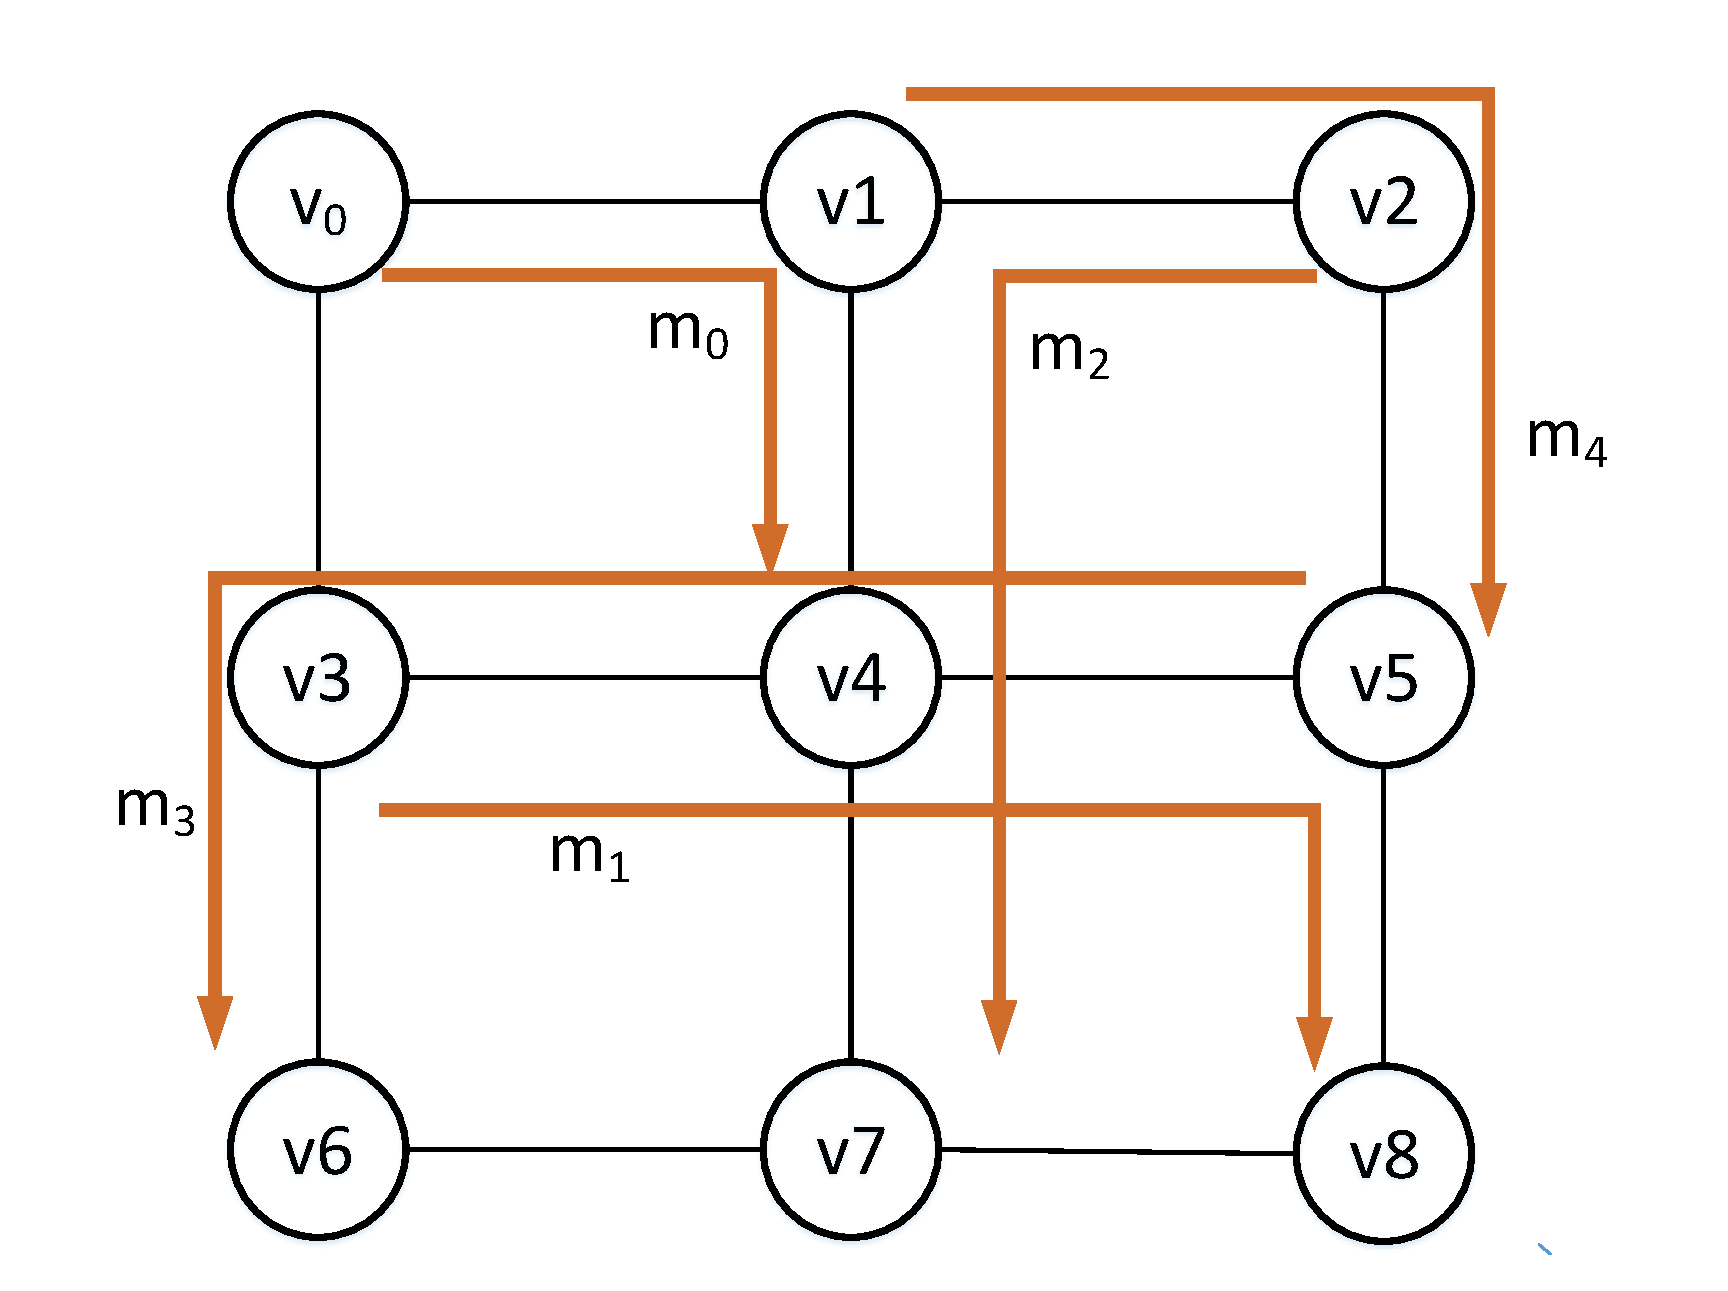
\includegraphics[width=2.5in]{picture/scheduling_example.pdf}
	\caption{An example of communication set on the TTNoC}
	\label{f:comm_on_TTNoC}
\end{figure}
\begin{table}[!t]
	\renewcommand{\arraystretch}{1.3}
	%if using array.sty, it might be a good idea to tweak the value of
	% \extrarowheight as needed to properly center the text within the cells
	\caption{An Example of a communication set $\mathcal{M}$}
	\label{t:comm_info}
	\centering
	% Some packages, such as MDW tools, offer better commands for making tables
	% than the plain LaTeX2e tabular which is used here.
	\begin{tabular}{|c||c||c||c||c|}
		\hline
		communication & link & period & delay & possible offset\\
		\hline
		$m_{0}$ & $ (0,4) $ & 2 & 1 & $\{0,1\}$\\
		\hline
		$m_{1}$ & $ (3,8) $ & 4 & 1 & $\{0,1,2,3\}$\\
		\hline
		$m_{2}$ & $ (2,7) $ & 4 & 1 & $\{0,1,2,3\}$\\
		\hline		
		$m_{3}$ & $ (5,6) $ & 8 & 2 & $\{0,1,2,3,4,5,6\}$\\
		\hline
		$m_{4}$ & $ (1,5) $ & 8 & 1 & $\{0,1,2,3,4,5,6,7\}$\\
		\hline		
	\end{tabular}
\end{table}

\subsection{Genetic Representation}

The genetic algorithm deployed as global search consists of gene, chromosome, individual and population. The population consists of a set of individual and each contains a chromosome which represents a solution to the given question. A chromosome composes of several gene, which as the unit of chromosome [wiki]. We will define them on the field of scheduling on TTNoC.

In our memetic algorithm, we adopt hyperperiod  $\mathcal{H(M)} = LCM\{\mathcal{M.T}\}$, which is the least common multiple among the set of period of communication set, as the chromosome definition. And the macrotick which is the unit of hyperperiod, is the gene. The length of chromosome equals $\mathcal{H(M)}$, e.g. the hyperperiod is 8 for the given example in TABLE. 

The location of a gene on the chromosome denotes the offset $ m_{i}^{(v_{a},v_{b})}.\phi $ of a communication scheduling $ {m_{i}^{(v_{a},v_{b})}\in\mathcal{M}} $. The offset of each communication is distributed on a gene. Therefore a chromosome represents a possible allocation of the offset set of the communication set $\mathcal{M}.\Phi$ It should be noted that a single gene may consists multiple offset of communication, since several communication is able to offset at same time based on the TTNoC architecture.

A set of individual with respective chromosome composes the population. The size of population equals the number of individual. An example of population with two individual, based on TABLE, is shown in Fig.

\begin{figure}[!t]
	\centering
	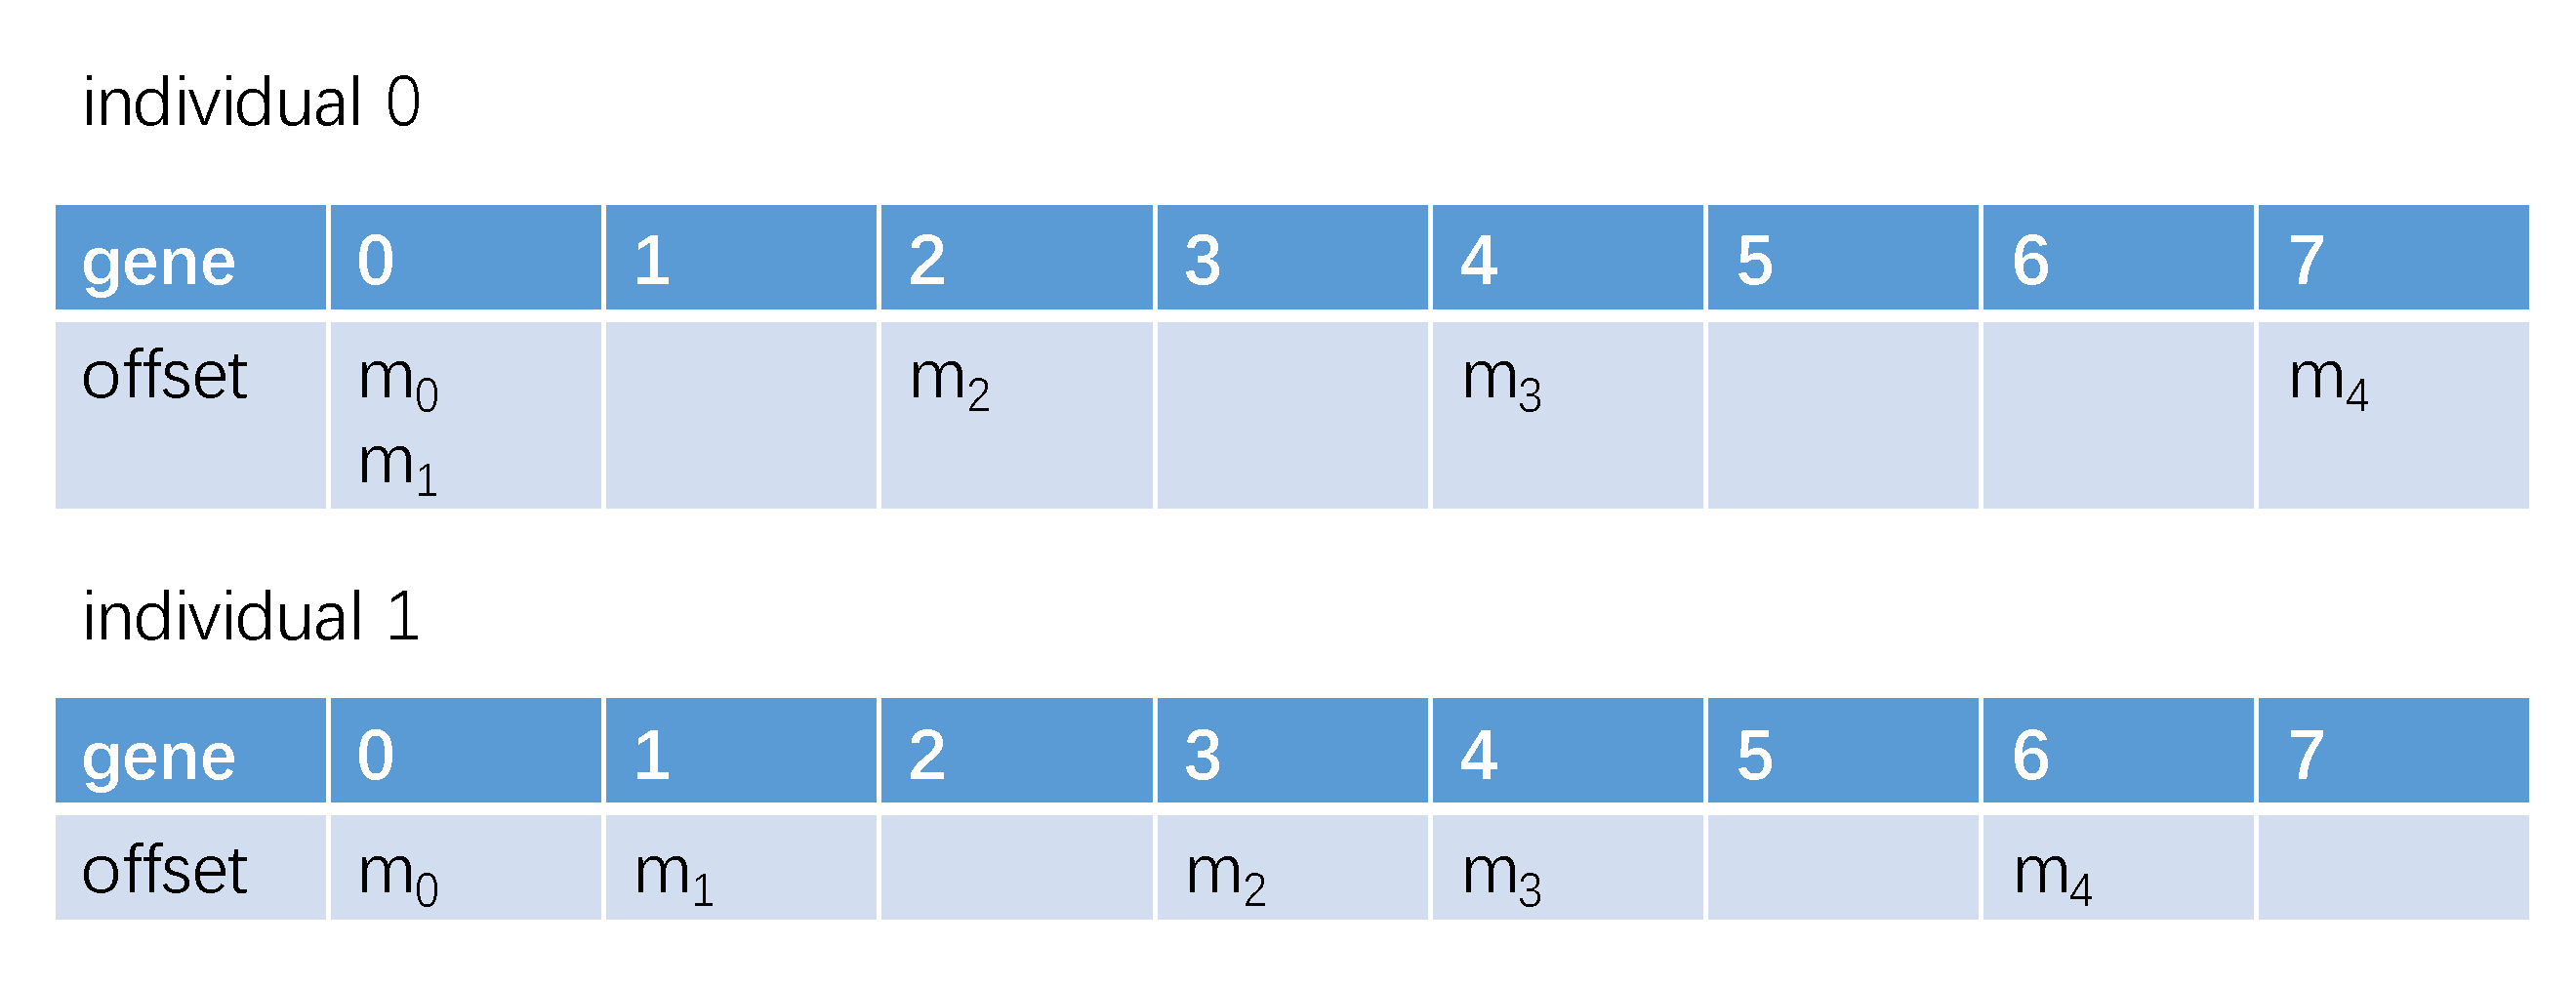
\includegraphics[width=3.5in]{picture/2individual}
	\caption{An example of population with 2 individual}
	\label{f:indi}
\end{figure}

\subsection{Pseudocode}

According to the genetic representation, we formal give the algorithm process. The pseudocode is given as follow.

The memetic algorithm begins with an initial population. The size of population as well as the maximum iterations is predefined. For a communication $m_{i}\in\mathcal{M}$, the offset of each communication $m_{i}.\phi$ in the initial individual is located randomly among the possible offset $m_{i}.\Phi$. Therefore the initial population satisfies the offset constrains. The algorithm is iterative executed until a feasible scheduling is found or reaching the given maximum iteration.

When the memetic algorithm get started, firstly the initial population is marked by the fitness function. The detail of fitness function is discussed in $subsection\ D$. Every time marking the population, a score is derived to evaluate each individual. And the less the number of score, the better the individual. Therefore the individual with score equals zero represent a feasible scheduling of the communication set.

Next, the operation of genetic algorithm, i.e. crossover and mutation, is deployed as global search. And after that, the local search is adopted to the population, if there are no feasible scheduling(individual with score of 0). The detail of search strategy deployed in global as well as local search, is discussed in $subsection\ E$ and $subsection\ F$, respectively.

After the global and local search, each individual in the population is evaluated by fitness function again. And the new population for the next iteration is generated by selection according to the score of each individual. The individual with less score own more possibility to reserve for the next population. The selection function ensure the size of population is equal to the predefined size in each iteration.

\begin{algorithm}[tb]
	\caption{Memetic Algorithm()}
	\renewcommand{\algorithmicrequire}{\textbf{Input:}}
	\renewcommand{\algorithmicensure}{\textbf{Output:}}
	\begin{algorithmic}[1]
		\REQUIRE~~\\
		the size of population $scale$\\
		maximum iterations $maxIteration$\\
		\ENSURE~~\\
		Best scheduling $\mathcal{S}$\\
		\FOR {$i = 0$ to $maxIteration-1$}
			\IF{$i=0$}
			\STATE // mark the initial population
				\STATE generate the	initial population $initialPop$\\
				\STATE mark$(initialPop)$
				\STATE $\mathcal{S}$ = individual with least score \textbf{in} $initialPop$
				\STATE $Pop = initialPop$
			\ELSE
			\STATE // global search
				\STATE crossover($Pop$)
				\STATE mutation($Pop$)
				\STATE mark$(Pop)$
			\ENDIF
			\STATE // choose the individual best so far after global search
			\FORALL {individual $indi$ \textbf{in} $Pop$}		
				\IF{$indi.score<\mathcal{S}.score$}
					\STATE $\mathcal{S}=indi$
				\ENDIF
				\IF{$\mathcal{S}.score==0$}
					\STATE break
				\ENDIF
			\ENDFOR	
			\STATE localSearch($Pop$)
			\STATE mark$(Pop)$
			\STATE // choose the individual best so far after local search
			\FORALL {individual $indi$ \textbf{in} $Pop$}		
				\IF{$indi.score<\mathcal{S}.score$}
					\STATE $\mathcal{S}=indi$
				\ENDIF
				\IF{$\mathcal{S}.score==0$}
					\STATE break
				\ENDIF
			\ENDFOR			
			\STATE select($Pop$, $scale$)
		\ENDFOR
		\RETURN {$\mathcal{S}$}
	\end{algorithmic}
\end{algorithm}	

\subsection{Fitness function}

To adopt the fitness function to evaluate individuals, we firstly transform chromosome representing the offset of each communication, into the representation of the duration of each communication in the hyperperiod. Next we derive the link constrains among the set of communication according to the routing strategy, as the basis of our fitness function. Then the score of each individual is able to derived by fitness function.

For each communication $m_{i}\in \mathcal{M}$, The duration of communication $m_{i}$ in $\mathit{k}$th period ${m_{i}^{(v_{a},v_{b})}}(k)$, is defined by formula (6). And we have that
\begin{equation}
m_{i}.\mathcal{H} = \{ {m_{i}^{(v_{a},v_{b})}}(k) \mid k \in [0, \mathcal{M.H} / m_{i}.\mathcal{T} - 1] \}
\end{equation}
where $m_{i}.\mathcal{H}$ denotes the duration in hyperperiod of a communication in hyperperiod.
We define $\mathcal{M.H}=\{ m_{i}.\mathcal{H} \mid m_{i}\in \mathcal{M} \}$, denotes the set of duration for each communication in hyperperiod. 
Therefore, the complete duration in hyperperiod for each communication $\mathcal{M.H}$ is determined based on the set of communications $\mathcal{M}$ . e.g. Fig~\ref{f:duration} is the complete duration in a hyperperiod based on the offset in Fig~\ref{f:indi} and the period as well as duration in TABLE~\ref{t:comm_info}.

\begin{figure}[!t]
	\centering
	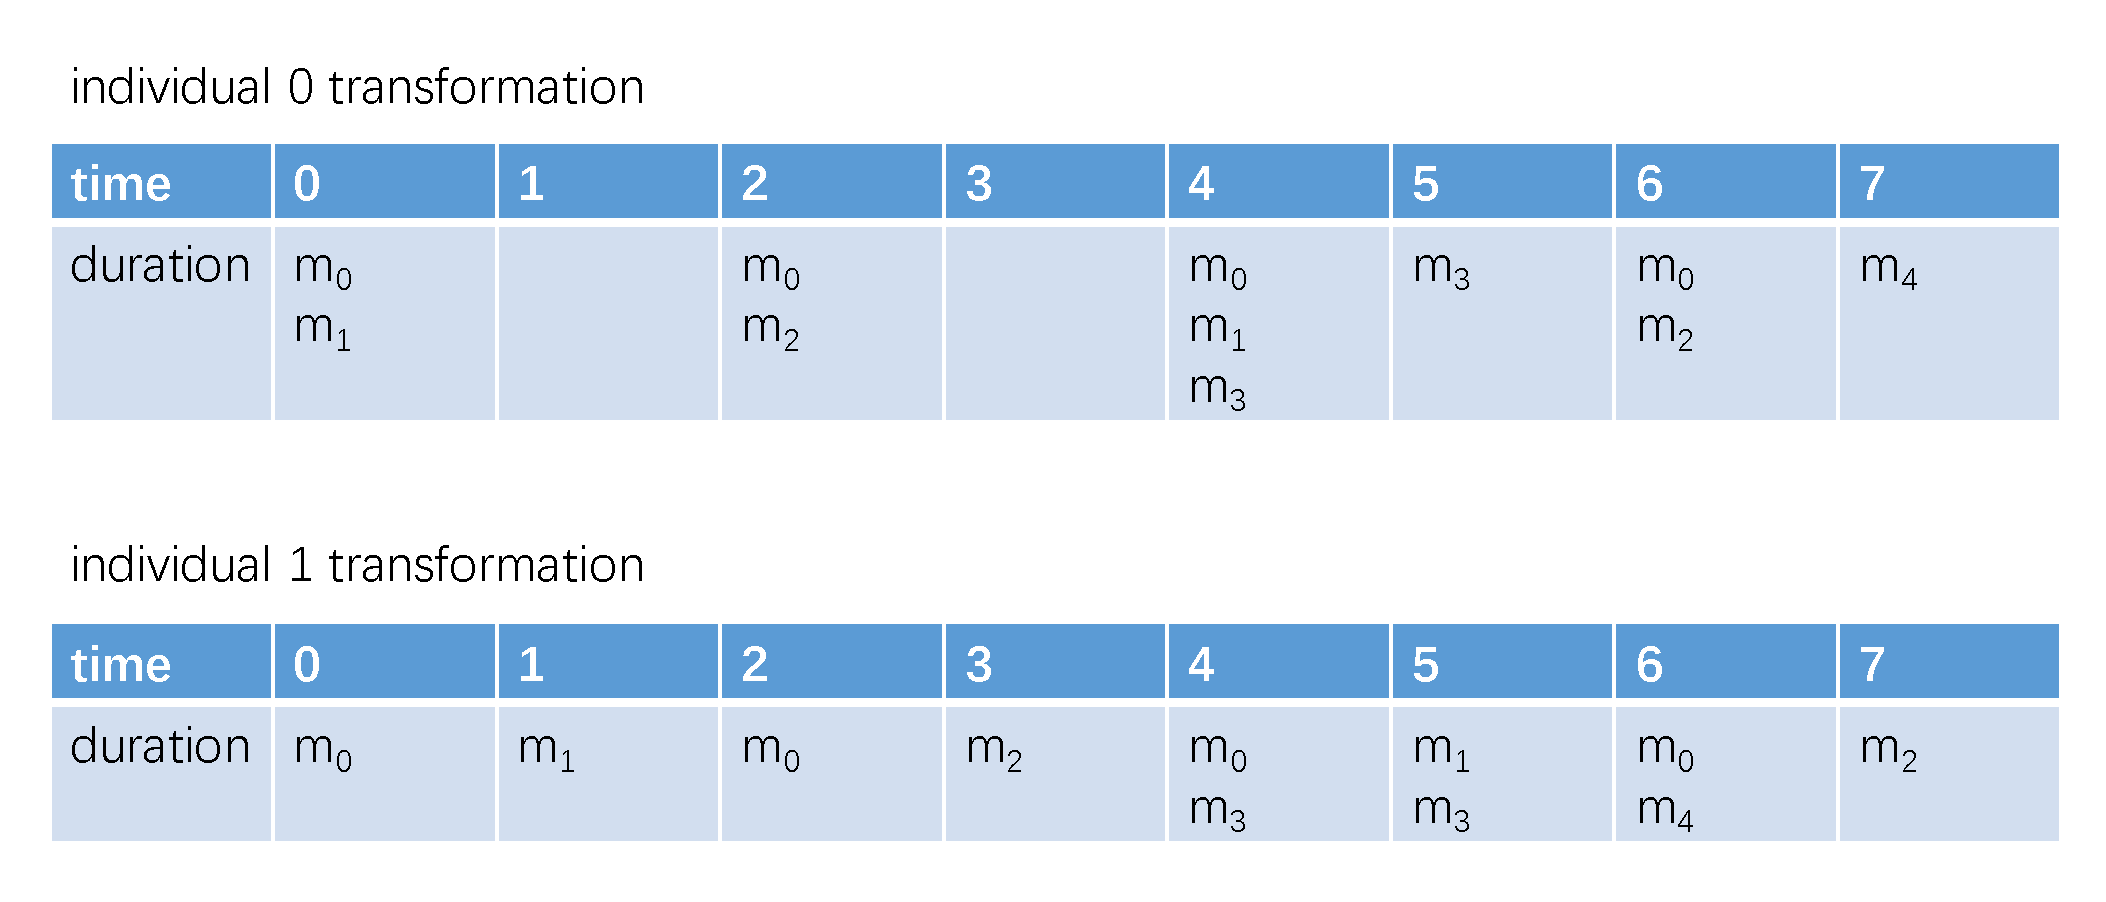
\includegraphics[width=3.5in]{picture/individual_transformation.pdf}
	\caption{The duration in the hyperperiod based on Fig and TABLE}
	\label{f:duration}
\end{figure}

The link constrains should be derived after the transformation of individual. According to the predefined routing strategy, i.e. XY routing, the network link $(v_{a},v_{b})$ of each communication $m_{i}\in\mathcal{M}$ is derived. Therefore we have the forwarding path per hop $ (v_{a},v_{b})=\{ <v_{a},v_{1}> ,\dots, <v_{i},v_{j}> ,\dots, <v_{n},v_{b}> \} $, where $m_{i}^{(a,b)}\in\mathcal{M}$. By checking the routing of each communication by formula (5) in link constrains, the set of overlapped communication for each $m_{i}\in\mathcal{M}$ is derived. We denote the overlapped set of communication $m_{i}\in \mathcal{M}$ by $O(m_i)$. And we have that
\begin{equation}
	O(m_i) = \{ m_j \mid overlap(m_i,m_j)=1,m_i,m_j\in\mathcal{M}  \}
\end{equation}

 i.e. the $overlap(m_{0},m_{1})=0$, $overlap(m_{0},m_{2})=1$, $overlap(m_{0},m_{3})=0$ and $overlap(m_{0},m_{4})=1$, thus overlap set $O(m_{0})$ is $\{ m_{2},m_{4} \}$. Table II shows the routing and overlapped communication for communications based on TABLE I.

\begin{table}[!t]
	\renewcommand{\arraystretch}{1.3}
	%if using array.sty, it might be a good idea to tweak the value of
	% \extrarowheight as needed to properly center the text within the cells
	\caption{An Example of a routing and overlap set for $\mathcal{M}$}
	\label{t:overlap}
	\centering
	% Some packages, such as MDW tools, offer better commands for making TABLEs
	% than the plain LaTeX2e tabular which is used here.
	\begin{tabular}{|c||c||c|}
		\hline
		communication & routing link & overlap set\\
		\hline
		$m_{0}$ & $ <0,1><1,4>$ 		& $m_{2},m_{4}$ \\
		\hline
		$m_{1}$ & $ <3,4><4,5><5,8>$	& $m_{4}$ \\
		\hline
		$m_{2}$ & $ <2,1><1,4><4,7>$ 	& $m_{0},m_{4}$ \\
		\hline		
		$m_{3}$ & $ <5,4><4,3><3,6>$ 	& \\
		\hline
		$m_{4}$ & $ <1,4><4,5>$ 		& $m_{0},m_{1},m_{2}$ \\
		\hline		
	\end{tabular}
\end{table}

To evaluate individuals, for $m_{i},m_{j}\in \mathcal{M}, m_{i}\neq m_{j}$, if two communication in the same overlap set, the conflict times between them are derived. We define the mapping $(m_{i},m_{j})\rightarrow n_{ij}$, where $(m_{i},m_{j})$ is the conflict communication and $n_{ij}$ is the number of gene which $m_{i}$ coexist with $m_{j}$ on a chromosome is $n_{ij}$, which denotes the conflict times between $m_{i}$ and $m_{j}$.

For each communication $m_{i}\in\mathcal{M}$, we define $C(m_{i})$ to derive the communication which conflicted with $m_{i}$ and the conflict times. Therefore we have that
\begin{equation}
	C(m_{i}) = 
\{(m_{i},m_{j})\rightarrow n_{ij}\mid m_j\in O(m_{i}),m_{i},m_{j}\in \mathcal{M}\}
\end{equation}

We define the total conflict times to $m_{i}$ as $C(m_i).value$. And we have that
\begin{equation}
	C(m_i).value=\sum n_{ij}
\end{equation}
If there is no conflict communication with $m_i$ on the transformation of individual , the value of $C(m_i)$ equals 0. We define $C(\mathcal{M}) = \{ C(m_i)\mid m_i\in\mathcal{M} \} $ to denote the conflict mapping set for all the communication set $\mathcal{M}$.

According to $C(m_{i})$ for each $m_{i}\in\mathcal{M}$, the conflict times among any two of communication on the chromosome is determined. The fitness function defined to give each individual a score when executing $mark(Pop)$ in line 5, 12, 24 of the memetic algorithm. The output of fitness function is the sum of $n_{ij}$ in $C(m_{i})$ for each communication $m_{i}\in\mathcal{M}$. Therefore for a individual $indi$ with $p$ communication, we have that
\begin{equation}
	fitness(indi)=\sum_{i=0}^p {C(m_i).value}
\end{equation}
where $m_i\in\mathcal{M}$. The score is assigned to the individual after fitness function. Since the score represents the conflict times, the less the score the better the individual. e.g. The $C(\mathcal{M})$ and the score of two individual is shown in Fig, based on the transformation in Fig and the overlap set in TABLE. 

\begin{table}[!t]
	\renewcommand{\arraystretch}{1.3}
	%if using array.sty, it might be a good idea to tweak the value of
	% \extrarowheight as needed to properly center the text within the cells
	\caption{An Example of marking two individual by fitness function}
	\label{f:fitness}
	\centering
	% Some packages, such as MDW tools, offer better commands for making TABLEs
	% than the plain LaTeX2e tabular which is used here.
	\begin{tabular}{|c||c||c|}
		\hline
		$C(\mathcal{M})$ of individual 0 & conflict mapping & score\\
		\hline 
		$C(m_{0})$ & $ (m_0,m_2)\rightarrow 2$ & \multirow{2}{*}{4} \\
		\cline{1-2}  
		$C(m_{2})$ & $ (m_2,m_0)\rightarrow 2$ & \\
                \hline
                \multicolumn{3}{|l|}{score}\\
		\hline
			\hline
			$C(\mathcal{M})$ of individual 1 & conflict mapping & score\\
			\hline 
			$C(m_{0})$ & $ (m_0,m_4)\rightarrow 1$ & 2 \\
			\hline  
			$C(m_{4})$ & $ (m_4,m_0)\rightarrow 1$	&  \\
			\hline	
	\end{tabular}	

\end{table}

\subsection{Global search strategy}

The general operation in genetic algorithm, i.e. crossover and mutation, is used in the step of global search. 

For operation of crossover, we select two of individual among the population the parent to join the crossover in terms of the score. The higher scores of the individual, the higher possibility to be selected as parent. the crossover generates a new individual and the chromosome of the new individual depends on the parent. The individual of parent with lower score own the higher possibility to determine the offset location on the chromosome. For the parent individual $indi0$ and $indi1$, we have the function
\begin{equation}
	possibility(indi0)=1-\frac{indi0}{indi0+indi1}
\end{equation}
to derive the possibility for each individual. e.g. Fig~\ref{f:crossover} shows an process of crossover. The individual 2 is generated by crossover based on the two individual in Fig~\ref{f:indi} as parent.
\begin{figure}[!t]
	\centering
	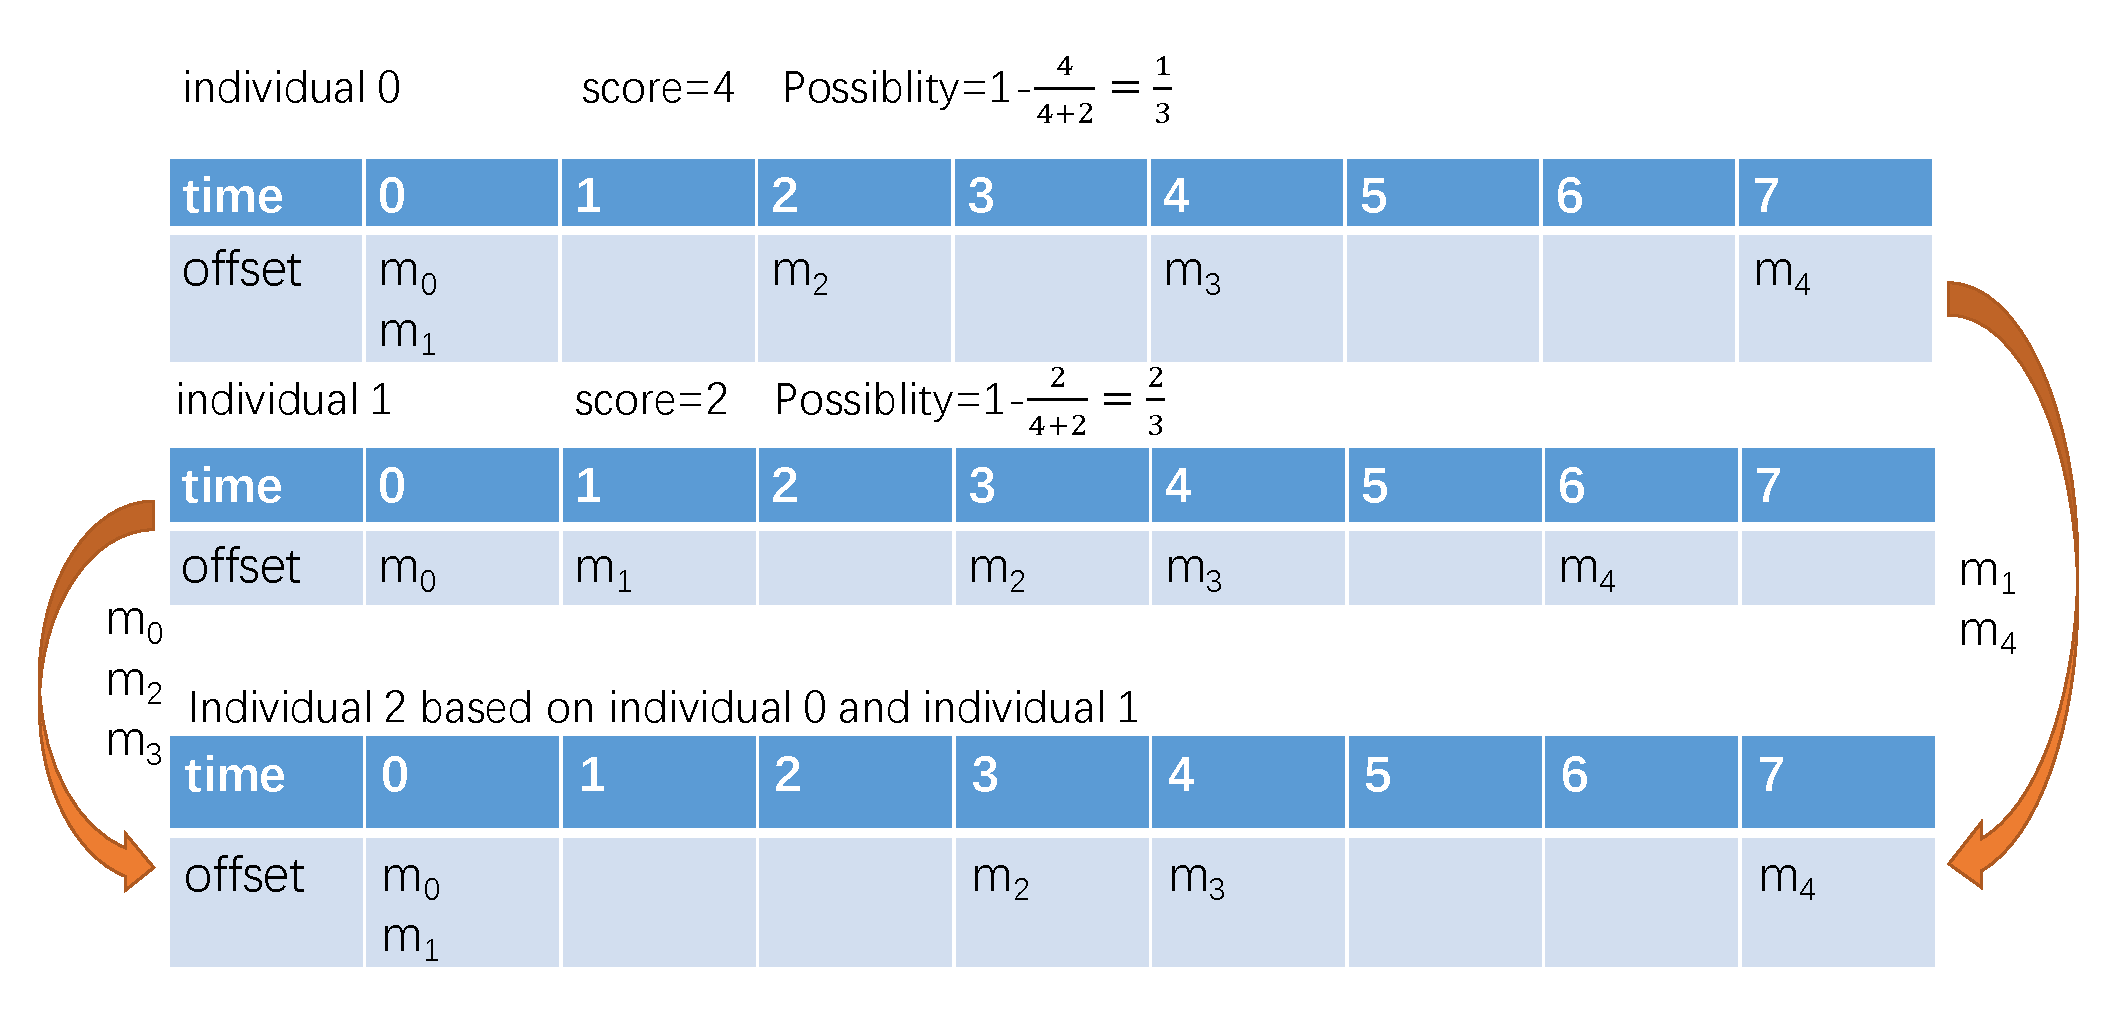
\includegraphics[width=3.5in]{picture/crossover.pdf}
	\caption{crossover}
	\label{f:crossover}
\end{figure}

The operation of mutation random select an offset of communication. Then selecting a new location of its offset randomly. Fig~\ref{f:mutation} is an example of mutation. The probability of mutation for each individual in our implement is 50\%.
\begin{figure}[!t]
	\centering
	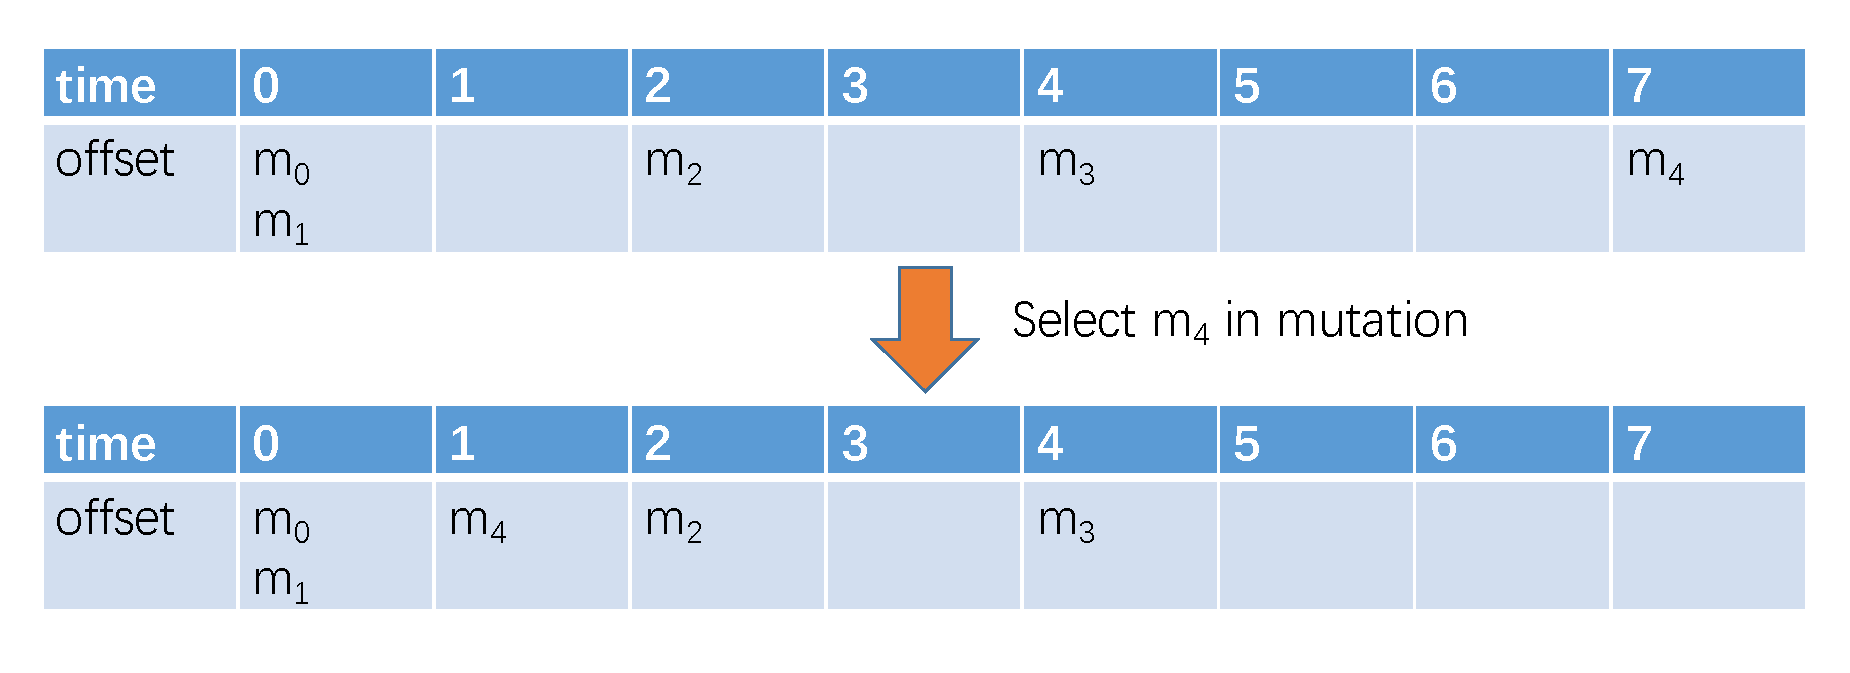
\includegraphics[width=3.5in]{picture/mutation.pdf}
	\caption{mutation}
	\label{f:mutation}
\end{figure}

\subsection{Local search strategy}

In the step of local search, for each individual, the communication $m_i$ with the maximum value of $C(m_i).value$ is selected as local search element. If there is two or more individual with the maximum conflict times, the element to be searched is select stochastically among them. After determining the element for local searching, the offset of selected $m_i$ is reallocated in its possible offset interval, to minimum the score of the individual.

Fig~\ref{f:local} shows an example of local search for $individual 0$ in Fig~\ref{f:indi}. According to the $C(\mathcal{M})$ of individual 0 in Fig~\ref{f:fitness}, we random select $m_0$ as the element. Since the possible offset of $m_0$ is 0 and 1 shown in TABLE I, we locate the $m_0$ on gene 0 and gene 1 respectively. After marking two of individual with different offset of $m_0$, we select the individual which score is 2 as the individual 0 because the score of individual 0' is minimum among the individual which just reallocate the offset of $m_0$.
\begin{figure}[!t]
	\centering
	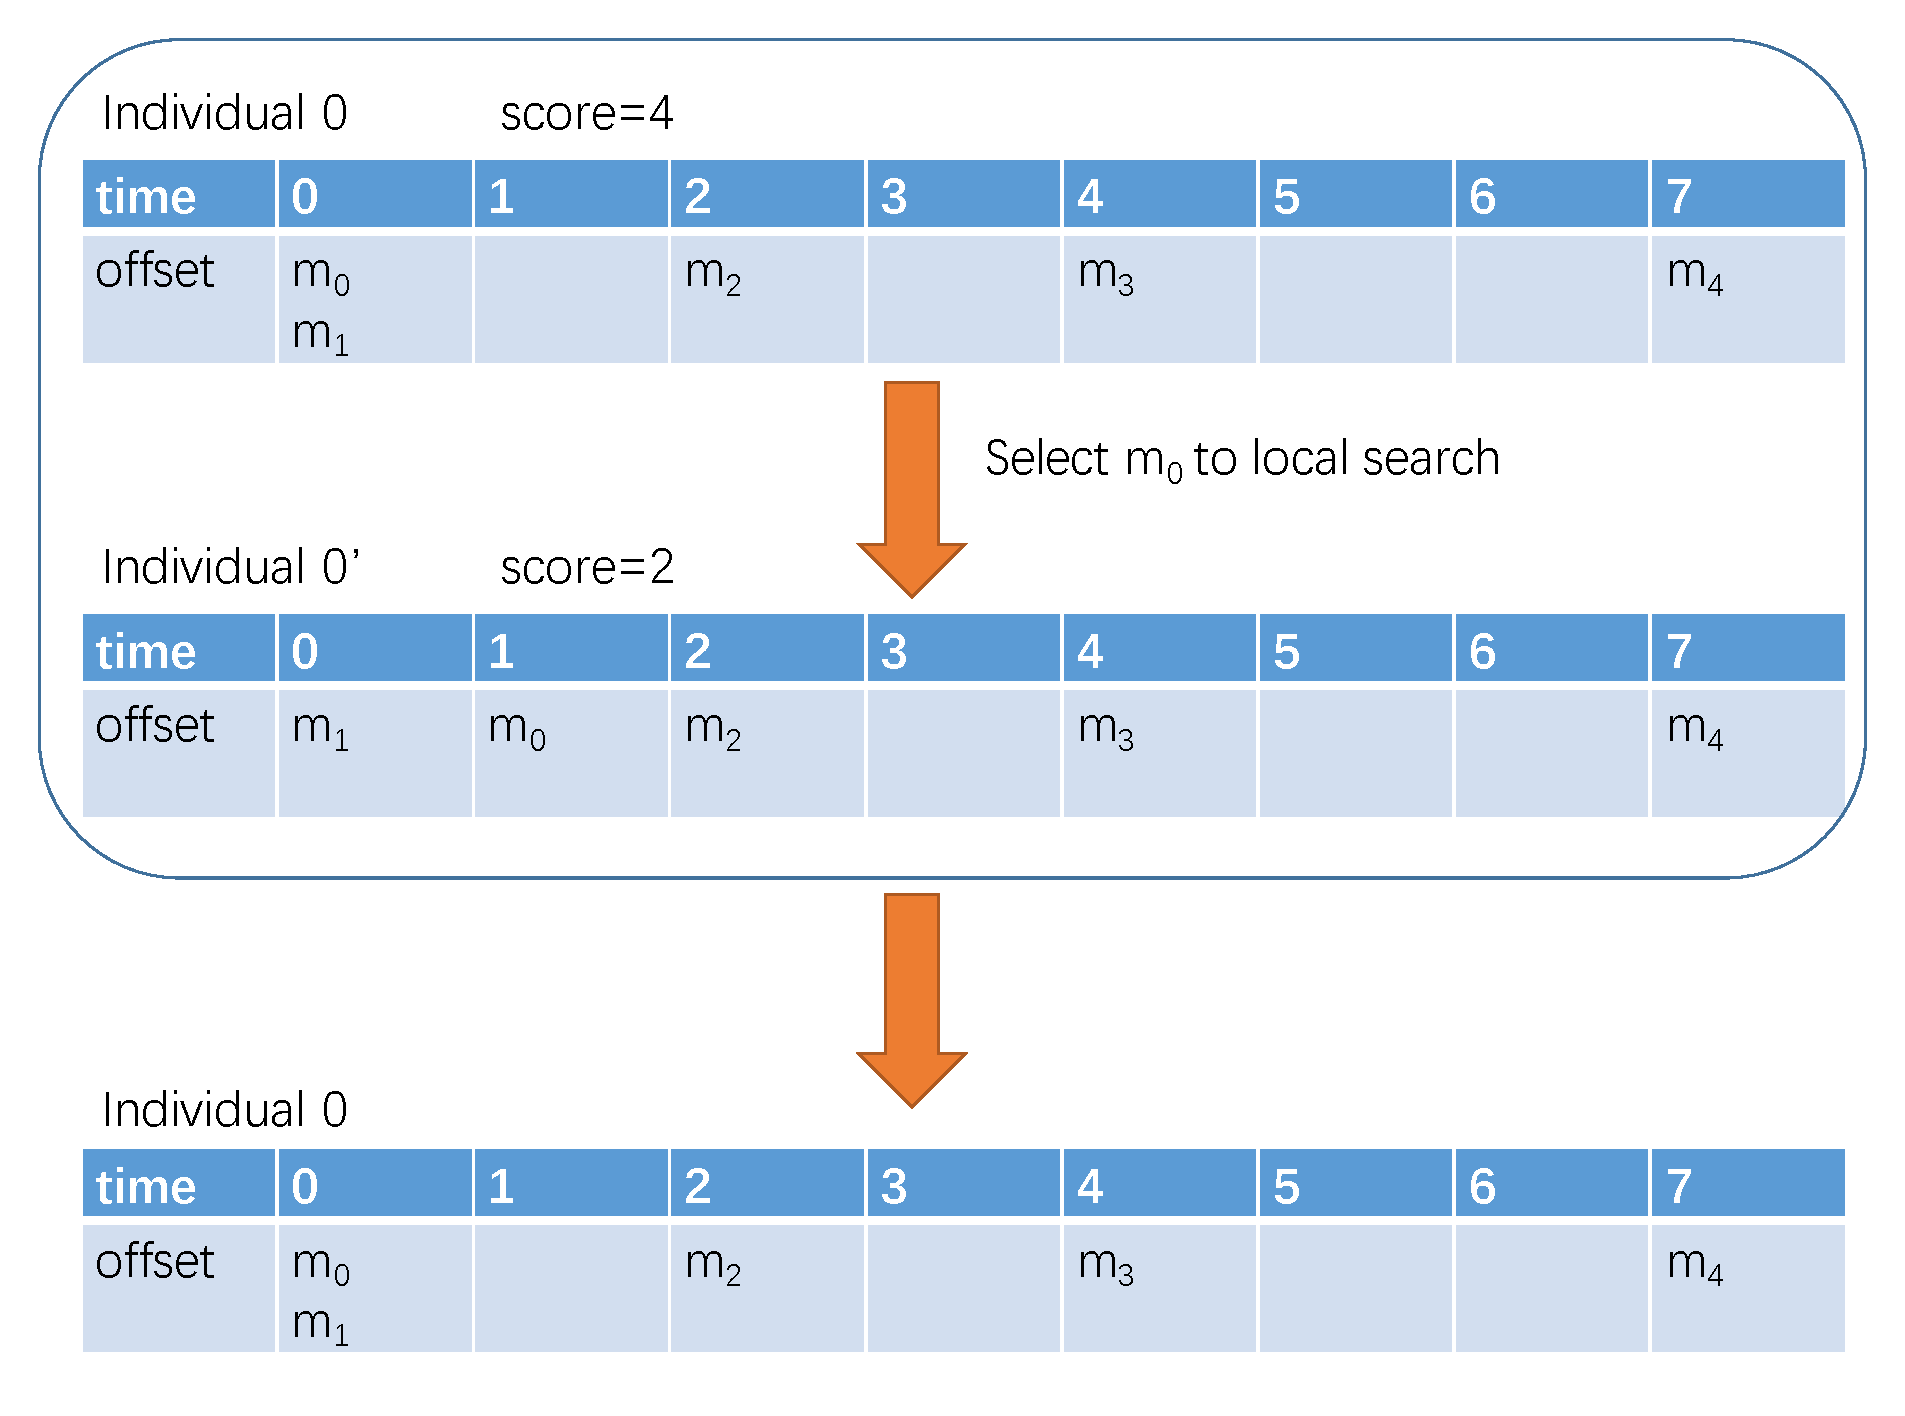
\includegraphics[width=3.5in]{picture/local.pdf}
	\caption{Local search fig}
	\label{f:local}
\end{figure}

In our implement, we naively traverse all the possible offset. However for improving efficiency, many other algorithm in local search can be applied, i.e. tabu search, simulated annealing. And different local search strategy may increase the performance of the memetic algorithm.

\section{EVALUATION}

\subsection{Experiments Configuration}

The network architecture we used is 2D mesh network which scale is $3\times 3$, $5\times 5$ and $7\times 7$, with 9, 25 and 49 switching nodes respectively. the program of our algorithm is implement in JAVA and is running on a Windows machine with 4GHz CPU and 12GB memory. We compare the memetic algorithm with general genetic algorithm without local search. 

We generate the set communication with different scale which from 5 to 50. Each communication owns its period and delay which is random generated. The size of population is 100. Therefore there is 100 initial individual. And the maximum iterate times is 100. The memetic algorithm will finish if there is a feasible scheduling, otherwise the algorithm will execute until the iterate 100 times. The case which executes exceeds an hour will be regarded as overtime.

\subsection{Failed Communication Percentage}
To compare the performance of the genetic algorithm and memetic algorithm, we define the failed communication as the minimum number of messages, which block the scheduling of other messages. in other word, if the set of failed communication is removed from the given communication set on the TTNoC, the remaining messages will be scheduled.

Fig shows the percentage of failed messages in the set of communication. For each type of case. As can be seen, though the general algorithm spends quite a few time, the rate of failed scheduled messages is much more than the memetic algorithm, especially when the scale of communication set is relatively large. i.e. for the case of 50 messages in $3\times 3$ TTNoC, the failed communication percentage is 17.3\% for genetic algorithm while 8\% for memetic algorithm. Therefore, the local search in the memetic algorithm is the key step in our algorithm and significantly improve the effect of genetic algorithm.

And it is clear that the failed communication rate decreases when the scale of TTNoC architecture is larger. The reason of this result is that the link resource increases with the growth of architecture and decrease the possibility of contention among the communication on the TTNoC. It also presents that the failed communication rate increases when the number of communication increasing. It is because that the limited link resources have to transmit more messages when there is more communication on the TTNoC.
\begin{figure}[!t]
	\centering
	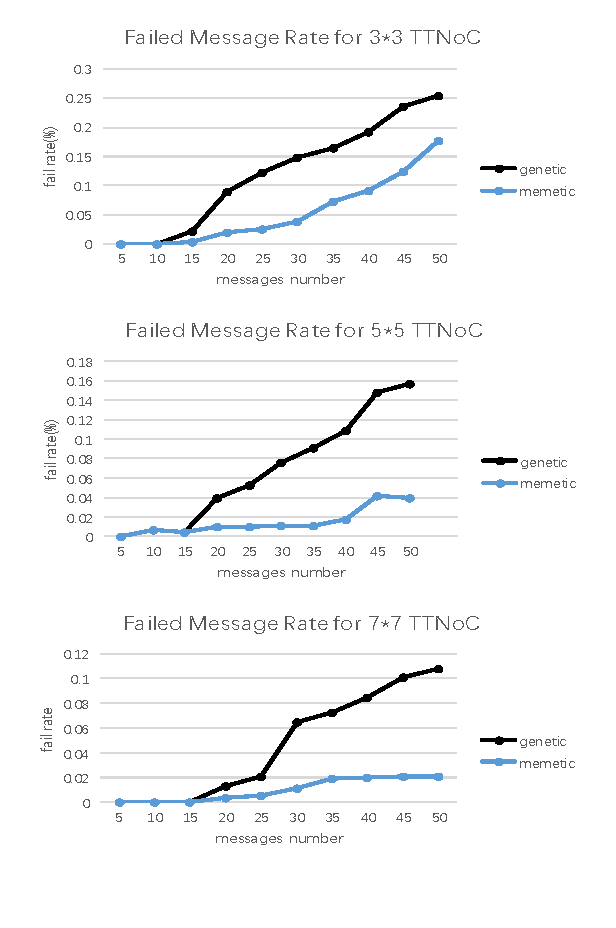
\includegraphics[width=3.5in]{picture/rate}
	\caption{fail rate}
	\label{f:fail}
\end{figure}

\subsection{Feasible Case}

We consider the number of feasible  case in each experiment type. For each test case, we define the case is successful if all the communication are scheduled in feasible location without link contention, otherwise we consider the case is infeasible case. A case is overtime is the case which synthesis time over 90 minutes. Fig presents the result of number of feasible cases after schedule synthesis. For simple test cases with less than 15 communication, almost cases is feasible. But for complexed test cases more than 30 communication, it is hard for the algorithms to find a feasible scheduling.
\begin{figure}[!t]
	\centering
	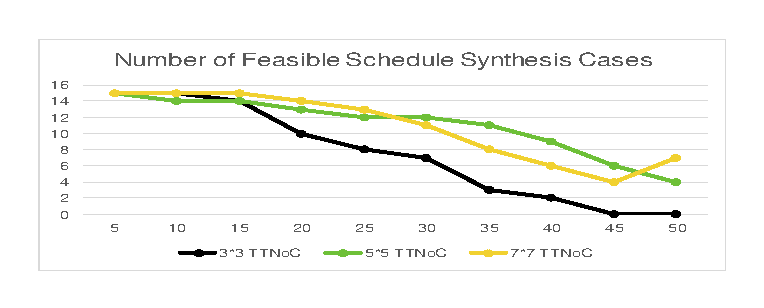
\includegraphics[width=3.5in]{picture/feasible}
	\caption{feasible case}
	\label{f:feasible}
\end{figure}

\section{FUTURE WORK}

Synthesizing a feasible scheduling depends on the number of communication and the scale of TTNoC. It is hard for memetic algorithm to synthesize a feasible scheduling when the set of communication is large and/or the TTNoC architecture is small. However, except of two reason above, the mapping between a message and a communication node and routing strategy of communications also affect generating a feasible solution. Therefore the designer can manually change the map allocation or the routing strategy to the failed messages, and even design a larger network architecture if needed, and after these change, the feasible scheduling can be generated by the memetic algorithm iteratively. 

Therefore the mapping between messages and nodes and routing strategy can be integrated to the TTNoC scheduling in our future work. And the different TTNoC architecture, i.e. torus, hypercube, and different local search strategy may be also considered in our experiment.

\section{CONCLUSION}

This paper introduces a memetic algorithm to resolve the message scheduling problem on the TTNoC for the real-time communication. We test our memetic algorithm with different scales of TTNoC and various messages. The experiment results shows that our memetic algorithm is efficient to synthesize a scheduling with low fail communication percentage.






% conference papers do not normally have an appendix


% use section* for acknowledgment
\section*{Acknowledgment}


The authors would like to thank...





% trigger a \newpage just before the given reference
% number - used to balance the columns on the last page
% adjust value as needed - may need to be readjusted if
% the document is modified later
%\IEEEtriggeratref{8}
% The "triggered" command can be changed if desired:
%\IEEEtriggercmd{\enlargethispage{-5in}}

% references section

% can use a bibliography generated by BibTeX as a .bbl file
% BibTeX documentation can be easily obtained at:
% http://mirror.ctan.org/biblio/bibtex/contrib/doc/
% The IEEEtran BibTeX style support page is at:
% http://www.michaelshell.org/tex/ieeetran/bibtex/
%\bibliographystyle{IEEEtran}
% argument is your BibTeX string definitions and bibliography database(s)
%\bibliography{IEEEabrv,../bib/paper}
%
% <OR> manually copy in the resultant .bbl file
% set second argument of \begin to the number of references
% (used to reserve space for the reference number labels box)
%% \begin{thebibliography}{1}

%% \bibitem{IEEEhowto:kopka}
%% H.~Kopka and P.~W. Daly, \emph{A Guide to \LaTeX}, 3rd~ed.\hskip 1em plus
%%   0.5em minus 0.4em\relax Harlow, England: Addison-Wesley, 1999.

%% \end{thebibliography}

\bibliographystyle{IEEEtran}
\bibliography{main}


% that's all folks
\end{document}


